%--------------------------------------------------
% INSTRUCTIONS / INSTRUÇÕES / INSTRUCCIONES
%--------------------------------------------------

% Este archivo es la plantilla oficial de la RBIE para artículos escritos en ESPAÑOL.

% Para português: use main-pt.tex
% For English: use main-en.tex

% No cambie la opción de idioma en \documentclass.

%----- MOTOR DE COMPILACIÓN
% Recomendado: XeLaTeX o LuaLaTeX
% NO añada \usepackage[utf8]{inputenc}: UTF-8 ya es nativo en LaTeX moderno y el paquete es obsoleto en esta plantilla.

%----- QUÉ EDITAR EN ESTE PREÁMBULO
% 1. \title / \engtitle -- título en español y su versión en inglés
% 2. \author{} -- nombres, ORCID y correos electrónicos

%----- REFERENCIAS
% 1. La norma bibliográfica APA 7.ª edición ya está definida en el estilo 'apalike-sol.bst'; NO LO CAMBIE.
% 2. Añada las entradas bibliográficas al archivo refs.bib

%-----  PAQUETES YA CARGADOS POR LA CLASE (no los redeclare):
    % algorithm, algpseudocode
    % amsmath, amssymb
    % babel
    % caption
    % cuted
    % enumitem
    % etoolbox
    % fontawesome
    % geometry
    % graphicx
    % hyperref
    % listings
    % microtype
    % minted
    % natbib
    % tcolorbox
    % titlesec
    % xcolor
%--------------------------------------------------



% ---- ACCESIBILIDAD: generacion de PDF etiquetado (tagged PDF / PDF/UA)
% Esta línea DEBE permanecer antes de \documentclass. Activa el marcado estructural automático exigido por las Pautas de Accesibilidad para el Contenido Web (WCAG) y por las orientaciones de accesibilidad de la Comisión para la Inclusión, la Diversidad y la Equidad (CIDE) de la Sociedad Brasileña de Computación (SBC): encabezados, listas, tablas y orden de lectura expuestos a los lectores de pantalla. Define además el idioma del PDF (/Lang) y el estándar PDF/UA-2 (ISO 14289-2), norma internacional de accesibilidad universal para archivos PDF.
% En TeX Live 2023 o anterior las claves 'tagging'/'pdfstandard' no existen y la compilacion falla: en ese caso, actualice la distribucion. Valide el PDF final (vease la seccion de figuras).
\DocumentMetadata{
  lang          = es,
  pdfversion    = 2.0,
  pdfstandard   = ua-2,
  tagging       = off
}

\documentclass[spanish]{rbie2026}%

% Controla el comportamiento y la posición de las notas al pie
\usepackage[bottom]{footmisc}

%% El paquete tabularray es el más moderno y completo disponible para la construcción de tablas. Reemplaza a los paquetes tabularx, multirow, multicol, colortbl y longtable
% https://ctan.org/pkg/tabularray
\usepackage{tabularray}

% Habilita los comandos clásicos de 'booktabs': \toprule, \midrule, \bottomrule y \cmidrule dentro del entorno tblr:
\UseTblrLibrary{booktabs}

% Formatea números y unidades según el Sistema Internacional de Unidades (SI)
\usepackage{siunitx}

%% Resalta código y demostraciones con l3regex y LPeg
% Habilita el comando \fakeverb{}, más robusto que el comando nativo \verb||
\usepackage{codehigh}

% Formatea las direcciones web en fuente monoespaciada
\usepackage{url}

% Evita líneas viudas y huérfanas
\clubpenalty  = 100000000
\widowpenalty = 100000000


%----- INFORMACIÓN DE ENCABEZADO. NO EDITAR -----------
%----- RESERVADO SOLO PARA LOS EDITORES
\jid{RBIE}
\jtitle{Revista Brasileira de Informática na Educação, 20XX, VV:1}
\issn{1414-5685 (print), 2317-6121 (online)}
\doi{10.5753/rbie.yyyy.id}
\copyrightstatement{This work is licensed under a Creative Commons Attribution 4.0 International License}
\jyear{20XX}

\category{Artigo de Pesquisa / Research Paper / Artículo de investigación}

    % --- Alternativas:
    % \category{Artigo estendido / Extended Paper / Artículo extendido}

    % \category{Edição Especial / Special Issue / Edición especial}

% número de página inicial
% \setcounter{page}{889}
%--------------------------------------------------


%----- ACCESIBILIDAD: metadatos del PDF (recomendado) -----
% Complete el titulo y las personas autoras en TEXTO SIMPLE (sin comandos LaTeX, sin colores, sin "--"). El lector de pantalla anuncia \pdftitle en lugar del nombre del archivo (ya habilitado por pdfdisplaydoctitle=true en la clase).
\hypersetup{pdftitle={Presentacion de la plantilla RBIE para 2026: versión para artículos en español},
            pdfauthor={Alexandre Direne; José Valente; Liane Tarouco}
            }

%----- TÍTULO DEL ARTÍCULO -------------------------------

% Título en español [Título corto]{Título largo}
\title[Título corto del artículo en español]{Presentación de la plantilla de la RBIE para 2026 -- versión para artículos en español}

% Título en inglés (versión secundaria)
\engtitle{\textcolor{engtitle}{Presenting the RBIE template for 2026 -- version for papers written in Spanish}}
%--------------------------------------------------


%----- INFORMACIÓN DE AUTORÍA ------------------------
%----- EL ORCID ES OBLIGATORIO PARA CADA AUTOR EN LA RBIE

%----- ENVÍO ANÓNIMO
% Para la revisión a doble ciego:
% 1. Comente todo el bloque \author{}
% 2. En el cuerpo del artículo, sustituya nombres y afiliaciones por texto neutro
% 3. Véase la Sección 3.3.1 para más detalles

\author[
    % Autor/año corto
    % Elija SOLO UNA de las tres opciones siguientes:
    Direne 20XX (1 autor) | Direne \& Tarouco 20XX (2 autores) | Direne et al. 20XX (3 o más autores)]{
    
    % Datos del autor 1
        \affil{\textbf{Alexandre Ibrahim Direne} \thinspace \orcidlink{0000-0000-0000-0000} \thinspace \textcolor{blue}{\faEnvelopeO} \enspace [{Universidade Federal do Paraná} \thinspace | \thinspace \href{mailto:alexd@inf.ufpr.br}{{\textit{alexd@inf.ufpr.br}}}]}
    
    % Datos del autor 2
        \affil{\textbf{José Armando Valente} \thinspace \orcidlink{0000-0002-1347-186X} \enspace [{Universidade Estadual de Campinas} \thinspace | \thinspace \href{mailto:jvalente@unicamp.br}{{\textit{jvalente@unicamp.br}}}]}
    
    % Datos del autor 3
        \affil{\textbf{Liane Margarida Rockenbach Tarouco} \thinspace \orcidlink{0000-0002-5669-588X} \enspace [{Universidade Federal do Rio Grande do Sul} \thinspace | \thinspace \href{mailto:liane@penta.ufrgs.br}{{\textit{liane@penta.ufrgs.br}}}]}
}
%--------------------------------------------------


\begin{document}

%----- Elementos pretextuales (front matter)

\begin{frontmatter}
    \maketitle

    % Dirección de correo del autor de correspondencia
    \begin{mail}
        Departamento de Informática, Centro Politécnico, Universidade Federal do Paraná, R. Evaristo F. Ferreira da Costa, 383--391, Jardim das Américas, Curitiba, PR, 81530-090, Brasil.
    \end{mail}

%----- Resumen y palabras clave
    % Los artículos en español proporcionan el resumen y las palabras clave en español (nativo) y en inglés.

    % Resumen en español
    \begin{abstract-es}
        \textit{Introducción.} Los procesos editoriales en las revistas científicas requieren un perfeccionamiento continuo para acompañar la evolución de las prácticas de investigación y las exigencias de transparencia y reproducibilidad. \textit{Métodos.} Este artículo presenta el nuevo modelo de artículo de la Revista Brasileña de Informática en la Educación -- \emph{Revista Brasileira de Informática na Educação} (RBIE), describiendo su estructura y sus recomendaciones metodológicas para los más diversos tipos de investigación en Informática en la Educación. El modelo fue desarrollado únicamente en el formato \LaTeX\, contemplando tres idiomas. \textit{Resultados.} El modelo consolida en un único documento convenciones que antes estaban dispersas en ejemplos anteriores, reduciendo inconsistencias de formato y simplificando la evaluación por pares. \textit{Discusión.} La adopción de este modelo contribuye a la estandarización editorial de la RBIE y a la mejora de la calidad metodológica de los artículos enviados. El resumen en portugués debe aparecer antes del resumen en inglés (\emph{abstract}), seguido por el resumen en español. El resumen debe contener entre 150 y 300 palabras.
    \end{abstract-es}

    % Palabras clave en español
    \begin{pclaves}
        Revista Brasileña de Informática en la Educación; Plantilla de artículo; Redacción científica. [Indique de 3 a 10 palabras clave que favorezcan la indexación y recuperación del artículo en las principales bases de búsqueda de publicaciones científicas. Utilice punto y coma como separador. Las palabras clave deben comenzar con mayúscula.]
    \end{pclaves}

    % Resumen en inglés
    \begin{abstract-en}
        \textit{Introduction.} Editorial processes in scientific journals require continuous improvement to keep pace with the evolution of research practices and the growing demands for transparency and reproducibility. \textit{Methods.} This article presents the new article template of the Brazilian Journal of Computers in Education -- \emph{Revista Brasileira de Informática na Educação} (RBIE), describing its structure and its methodological recommendations for the most diverse types of research in Computers in Education. The template was developed only in the \LaTeX\ format, covering three languages. \textit{Results.} The template consolidates into a single document conventions that were previously scattered across earlier examples, reducing formatting inconsistencies and simplifying peer review. \textit{Discussion.} The adoption of this template contributes to RBIE's editorial standardization and to the improvement of the methodological quality of submitted articles. For papers written primarily in English, only the abstract in English is required. The abstract should contain between 150 and 300 words.
    \end{abstract-en}

    % Palabras clave en inglés
    \begin{keywords}
        Brazilian Journal of Computers in Education; Article template; Scientific writing. [Provide 3 to 10 keywords that facilitate the indexing and retrieval of the article in the main scientific publication databases. Please use semicolons as separators. Keywords must begin with capital letters.]
    \end{keywords}

% FECHAS DE EDICIÓN. NO EDITAR. RESERVADO SOLO PARA LOS EDITORES
    \begin{dates}
        {\sffamily\textbf{Received:}} DD Month YYYY \enspace\textbullet\enspace
        {\sffamily\textbf{Accepted:}} DD Month YYYY \enspace\textbullet\enspace
        {\sffamily\textbf{Published:}} DD Month YYYY
    \end{dates}

\end{frontmatter}

%----- Fin de los elementos pretextuales



%------ Inicio del texto del manuscrito
\section{Introducción a la Plantilla de Artículos de la RBIE}
\label{sec:intro}

Solicitamos a los autores interesados en enviar su investigación a la Revista Brasileña de Informática en la Educación (RBIE) que sigan las directrices de esta plantilla para garantizar una presentación estandarizada. Lea esta guía con atención, ya que presenta información importante sobre ética, orientaciones metodológicas e instrucciones de formato. Los manuscritos que no estén en el formato adecuado podrán ser rechazados por los editores en cualquier momento del proceso de revisión y publicación.

Los nombres de los autores que figuran en esta plantilla son un homenaje póstumo a tres investigadores que dedicaron su trayectoria al desarrollo de la Informática en la Educación en Brasil; ninguno de ellos participó en su elaboración.

\subsection{Alcance de la RBIE}

La RBIE tiene como objetivo difundir herramientas, métodos y prácticas que apoyen el uso eficaz de la tecnología en el proceso educativo. Aunque la RBIE se centró originalmente de forma exclusiva en la investigación en el área de Informática en la Educación, ahora también acoge y publica investigaciones en el área de Educación en Computación.

A pesar de compartir algunas características comunes, es importante establecer las diferencias entre las áreas de Informática en la Educación y Educación en Computación. Como señala \cite{Bispo2020}, la investigación en Informática en la Educación se refiere al uso de artefactos tecnológicos como mediadores en los procesos de enseñanza y aprendizaje, así como a sus impactos. La Educación en Computación, por su parte, tiene como objetivo principal la mejora de la enseñanza y el aprendizaje de la Computación como ciencia \citep{holmboe2001research}.


\subsection{Recomendaciones para Redactar la Sección de Introducción}

La sección de ``Introducción'', o un título equivalente, debe contextualizar el problema de investigación, identificar la laguna que el trabajo pretende cubrir y exponer explícitamente las contribuciones del artículo. Recomendamos la siguiente organización típica \citep{ecarnort_writing_article_2015}:

\begin{enumerate}
  \item \textbf{Contextualización (lo conocido).} Presente el escenario en el que se sitúa el problema, apoyándose en evidencias de la literatura. Evite afirmaciones genéricas sin respaldo bibliográfico.

  \item \textbf{Problema y laguna (lo desconocido).} Delimite el problema específico investigado y señale lo que la literatura aún no ha respondido plenamente. La laguna debe demostrarse, no simplemente declararse.

  \item \textbf{Objetivo y preguntas de investigación.} Exponga el objetivo general del trabajo. Cuando corresponda, presente las preguntas de investigación (PI) de forma explícita y numerada. Se trata de una práctica bien establecida en Informática en la Educación que facilita la evaluación de los revisores.

  \item \textbf{Contribuciones.} Enumere de forma concisa las principales contribuciones del trabajo. El uso de listas (\texttt{\textbackslash begin\{itemize\}} o \texttt{\textbackslash begin\{enumerate\}}) es aceptable en este punto, a criterio de los autores.

  \item \textbf{Organización del artículo.} Opcionalmente, describa en un párrafo final cómo se estructuran las secciones restantes del manuscrito.
\end{enumerate}

En el caso de artículos de revisión o de mapeo sistemático, la introducción debe incluir además la justificación para realizar una revisión secundaria sobre el tema, demostrando que no existe una revisión equivalente reciente o que la revisión existente presenta limitaciones relevantes.

Estas recomendaciones estructurales no son rígidas y pueden adaptarse a las características específicas de cada trabajo de investigación.


%------------------------------------------
\section{Instrucciones Específicas para \LaTeX}
\label{sec:latex}

La clase \texttt{rbie2026} está diseñada para trabajar con los motores \texttt{XeLaTeX} y \texttt{LuaLaTeX}. Por lo tanto, el documento debe compilarse:

\begin{enumerate}
    \item En Overleaf. Acceda a \textbf{Menú $>$ Configuración $>$ Compilador} y ajuste la opción ``Compilador'' a \texttt{XeLaTeX} o \texttt{LuaLaTeX}.\footnote{Los motores base se denominan \texttt{XeTeX} y \texttt{LuaTeX}. La combinación de estos motores con las macros de \LaTeX\ forma \texttt{XeLaTeX} y \texttt{LuaLaTeX}.}

    \item En su instalación local. Configure el editor o IDE (por ejemplo, TeXstudio, TeXworks o VS~Code) para utilizar \texttt{XeLaTeX} o \texttt{LuaLaTeX} como compilador. Como alternativa, compile desde la terminal con \texttt{xelatex archivo} o \texttt{lualatex archivo}. No es necesario indicar la extensión \texttt{.tex}.
\end{enumerate}

La clase \texttt{rbie2026} no funciona plenamente con el motor \texttt{pdfLaTeX}. Si intenta usarlo para compilar, recibirá mensajes de advertencia sobre paquetes de fuentes no definidos, y el PDF se generará con glifos ausentes en los iconos del paquete \texttt{fontawesome}, que depende de fuentes Unicode no compatibles con el motor \texttt{pdfLaTeX}.


\subsection{Diferencias entre \texttt{fontenc} y \texttt{fontspec}}

Los paquetes \texttt{fontenc} y \texttt{fontspec} controlan el manejo de fuentes y caracteres en \LaTeX. Pertenecen a épocas y motores de compilación distintos: \texttt{fontenc} se utiliza con el motor clásico (\texttt{pdfLaTeX}), mientras que \texttt{fontspec} es obligatorio para los motores modernos basados en Unicode (\texttt{XeLaTeX} o \texttt{LuaLaTeX}).

La distribución \textbf{TeX Live}, utilizada por Overleaf para preparar documentos \LaTeX, instala una amplia variedad de fuentes: por ejemplo, \textit{TeX Gyre Termes}\footnote{\url{http://www.gust.org.pl/projects/e-foundry/tex-gyre}} es el equivalente libre y abierto de la fuente \textit{Times New Roman}. Para los motores \texttt{XeLaTeX} o \texttt{LuaLaTeX}, no es obligatorio incluir el paquete \texttt{fontspec}. Omitirlo hace que el motor asuma valores predeterminados para la fuente y sus propiedades\footnote{Por simplicidad, el término \textsc{fuente} se emplea como sinónimo del término \textsc{tipo de letra}. No obstante, los profesionales de la tipografía distinguen entre ambos términos.}.


%------------------------------------------
\section{Organización del Manuscrito}
\label{sec:organization}

El manuscrito debe contener \textbf{entre 10 y 20 páginas}, excluyendo las declaraciones complementarias, las referencias y los apéndices.


\subsection{Configuración de la Página}

El tamaño del papel debe ser A4 (210 x 297 mm). Los márgenes del documento deben tener las siguientes medidas:

\begin{itemize}
    \item Superior: 1,0 cm
    \item Inferior: 2,0 cm
    \item Izquierdo: 1,8 cm
    \item Derecho: 1,7 cm
\end{itemize}

Estos valores ya están configurados en esta plantilla. No cambie las dimensiones de los márgenes, ya que cualquier texto fuera del estándar puede retrasar o incluso impedir la publicación de su artículo en la RBIE.


\subsection{Títulos}


\begin{table*}[ht]
    \centering
    \caption{Ejemplos de formato de título.}
    \label{tab:titulo}
    \begin{tblr}{%
        colspec = {ll},
        cells   = {font=\small}
        }
        \toprule
        \textbf{Incorrecto} & \textbf{Correcto} \\
        \midrule
        APRENDIZAJE DE PROGRAMACIÓN CON JUECES EN LÍNEA
            & Aprendizaje de Programación con Jueces en Línea \\
        aprendizaje de programación con jueces en línea
            & Aprendizaje de Programación con Jueces en Línea \\
        Aprendizaje De Programación Con Jueces En Línea
            & Aprendizaje de Programación con Jueces en Línea \\
        \bottomrule
        \end{tblr}
\end{table*}


Las recomendaciones que se presentan a continuación sobre la preparación de títulos se dividen en dos tipos: cómo elegir las palabras más adecuadas y cómo formatear su escritura.

\subsubsection{Elija un Título Atractivo}

Elabore un título estratégico que describa el alcance, el diseño y el objetivo del estudio. Recomendamos los siguientes consejos \citep{herbst2024structuring,ecarnort_writing_article_2015}:

\begin{enumerate}
  \item \textbf{Sea conciso y claro.} El título debe ser breve y directo, permitiendo que el lector infiera rápidamente el contenido de la publicación.

  \item \textbf{Evite formulaciones vagas.} Evite términos que no aporten valor informativo, como ``un informe sobre\ldots'' o ``un estudio acerca de\ldots''. Si los efectos son importantes, el título debe indicar exactamente cuáles son.

  \item \textbf{Identifique el diseño del estudio.} Los tipos específicos de diseño, como las revisiones sistemáticas, los mapeos sistemáticos y los experimentos controlados, deben identificarse explícitamente en el título.

  \item \textbf{Destaque el hallazgo principal.} Siempre que sea posible, el título debe indicar si la intervención aumenta, reduce o previene algo.

  \item \textbf{Ponga primero el aspecto más importante.} Si el foco es la intervención o la herramienta investigada, comience el título por ese elemento para distinguir el artículo de otros sobre el mismo tema.

  \item \textbf{Utilice palabras clave.} El título debe contener los términos principales para que el artículo pueda recuperarse fácilmente en bases de datos como SBC-OpenLib (SOL), ACM Digital Library, IEEE Xplore y Scopus.

  \item \textbf{Despierte interés.} El título debe ser lo bastante atractivo como para animar al posible lector a acceder al trabajo completo.

  \item \textbf{Diferencie su trabajo.} El título debe dejar claro cómo contribuye el artículo a la literatura o qué laguna del conocimiento del campo cubre.

  \item \textbf{Identifique revisiones y mapeos sistemáticos.} En el caso de estudios secundarios y terciarios, el título debe identificar si el artículo aborda un mapeo sistemático (o una revisión sistemática), un estudio terciario, una actualización de una revisión sistemática existente, o si incluye un metaanálisis \cite{Kitchenham2023_SEGRESS_supp}.
\end{enumerate}


\subsubsection{Formatee el Título} \label{sec:formatacao_titulo}

El título del manuscrito debe seguir estas convenciones de formato:

\begin{enumerate}
  \item \textbf{Formato tipográfico.} Para el título en el idioma original, utilice la fuente \textit{Roboto}, tamaño 18pt, alineada a la izquierda, con interlineado de 20pt y estilo negrita. Si el idioma original del manuscrito es el portugués o el español, los títulos en los idiomas secundarios deben usar la fuente \textit{Roboto}, tamaño 14pt, alineada a la izquierda, interlineado de 12pt, negrita y cursiva, en gris (RGB 128, 128, 128).

  \item \textbf{Uso de mayúsculas (\textit{title case}).} El título debe escribirse con solo la letra inicial de cada palabra en mayúscula. Deben llevar inicial \textbf{mayúscula}: la primera palabra del título (siempre); los sustantivos, adjetivos, verbos y adverbios; y los nombres propios, incluidos los nombres de sistemas, herramientas y plataformas (por ejemplo, Python, Moodle). Deben permanecer en \textbf{minúscula} (salvo cuando inician el título): los artículos (el, la, un, una); las preposiciones cortas (de, en, con, por, para); y las conjunciones (y, o, pero, que, si).

  \item \textbf{No se permite todo en mayúsculas.} El título no debe escribirse enteramente en mayúsculas, ni siquiera para enfatizar el trabajo. La Tabla~\ref{tab:titulo} presenta ejemplos de formato de título incorrecto y correcto.

  \item \textbf{Evite las siglas.} El título debería, idealmente, estar libre de siglas para garantizar la claridad y la accesibilidad para el lector no especialista.

  \item \textbf{No termine con punto.} Los títulos no forman parte del texto corrido, por lo que no deben terminar con un punto.
\end{enumerate}



\subsection{Información sobre los Autores}

Para la información de autoría (nombre, ORCID, afiliación, correo electrónico), utilice la fuente \textit{Roboto}, tamaño 10pt, alineada a la izquierda, con interlineado de 8pt y estilo normal, sin espaciado adicional.

Durante la fase de envío del manuscrito, debe suprimirse toda la información que pueda identificar la autoría. Si el trabajo es aceptado, esta información debe completarse tanto en los metadatos del formulario de envío como en la versión final del texto del manuscrito.


\subsubsection{Anonimización del Manuscrito}

Para garantizar la integridad de la revisión doblemente anonimizada, observe estas recomendaciones para la primera versión que se enviará:

\begin{itemize}
    \item \textbf{Autores y afiliaciones.} Omita los nombres, las afiliaciones institucionales y las direcciones de todos los autores. Los campos correspondientes en la plantilla deben completarse con \textit{Omitido para revisión}.

    \item \textbf{Agradecimientos.} Suprima la sección de agradecimientos, ya que a menudo identifica a financiadores, tutores o proyectos vinculados a los autores.

    \item \textbf{Financiación y ayudas.} No mencione agencias de financiación, números de proceso ni proyectos de investigación que puedan identificar a los autores o a sus instituciones.

    \item \textbf{Ubicación de los experimentos.} No mencione la ciudad donde se realizaron los experimentos o la recolección de datos. Mencione el estado o la región solo si esa información es relevante para la evaluación del mérito.

    \item \textbf{Plataformas y sistemas institucionales.} No mencione los nombres de plataformas, sistemas, entornos virtuales de aprendizaje o herramientas desarrolladas por los propios autores que puedan identificarlos. Cuando sea necesario, utilice designaciones genéricas, como \textit{el juego utilizado} o \textit{la plataforma de envío adoptada}.

    \item \textbf{Enlaces y URL.} No incluya hipervínculos que contengan información identificadora, como nombres de usuario, nombres de repositorios personales o institucionales, o dominios institucionales. Los repositorios de datos o de material complementario deben anonimizarse mediante servicios como \textit{Anonymous GitHub} (\url{https://anonymous.4open.science/}) antes del envío.

    \item \textbf{Autocitas.} Al citar su propio trabajo, utilice una formulación neutra como \textit{[omitido para revisión]} en lugar de la referencia bibliográfica, evitando expresiones como \textit{``como demostramos en [X]''} o \textit{``en un trabajo anterior, investigamos...''}.

    \item \textbf{Metadatos del archivo.} Verifique y elimine los metadatos del archivo PDF antes del envío, ya que pueden contener el nombre del autor, la institución o el software utilizado para la edición. En Linux, el comando \texttt{exiftool -{}-all= archivo.pdf} realiza esta limpieza; en Windows y macOS, el mismo resultado puede obtenerse a través de las propiedades del documento.

    \item \textbf{Figuras y capturas de pantalla.} Asegúrese de que las imágenes, los diagramas y las capturas de pantalla no muestren logotipos institucionales, nombres de usuario, direcciones de correo electrónico ni ningún otro elemento identificador.

    \item \textbf{Cuestionarios e instrumentos de investigación.} Si el manuscrito describe instrumentos y cuestionarios aplicados en una institución específica, elimine (o generalice) las referencias al contexto institucional en la redacción y en los ejemplos reproducidos en el texto.
\end{itemize}


\subsubsection{Restauración de la Autoría tras la Aceptación del Manuscrito}

Tras la aceptación definitiva del manuscrito, envíe la versión final con toda la información restaurada, incluidos los nombres, las afiliaciones, los agradecimientos y las referencias completas. Para cada autor, la información debe presentarse en la siguiente secuencia:

\begin{enumerate}
    \item Nombre completo de la persona, sin abreviaturas

    \item Enlace al perfil de ORCID (\textit{Open Researcher and Contributor ID})\footnote{\url{https://orcid.org/}}.

    \item Cuando corresponda, indique el autor de correspondencia mediante el símbolo \textcolor{blue}{\faEnvelopeO}.

    \item Nombre de la institución a la que está afiliado el autor.

    \item Dirección de correo electrónico.
\end{enumerate}


\subsection{Resumen y Palabras Clave}

El resumen es la sección más leída de un artículo científico. Probablemente será la única que se lea antes de decidir si se lee el trabajo completo. Debe ofrecer una visión general del manuscrito, abarcando sus objetivos, la metodología, los principales resultados y las conclusiones. A continuación se presentan algunas recomendaciones para planificar la estructura del resumen, refinar su lenguaje y estilo, eliminar errores comunes y darle formato.


\subsubsection{Planificación de la Estructura del Resumen}

Planifique y estructure el contenido del resumen antes de desarrollar las frases, siguiendo las orientaciones que se detallan a continuación \citep{ecarnort_writing_article_2015}:

\begin{enumerate}
  \item \textbf{Redáctelo al final.} Escriba el resumen después de completar todas las demás secciones del manuscrito, ya que solo entonces es posible sintetizarlo con precisión.

  \item \textbf{Hágalo autocontenido.} El resumen debe funcionar como un documento independiente: el lector debe comprenderlo plenamente sin necesidad de consultar el texto completo.

  \item \textbf{Adopte el formato IMRAD.} Recomendamos adoptar la estructura estándar compuesta por Introducción, Métodos, Resultados y Discusión (IMRAD) \citep{abstract_Nundy2022}.

  \item \textbf{Responda cuatro preguntas fundamentales:}
  \begin{enumerate}
    \item ¿Por qué empezó? (Introducción/Objetivo)
    \item ¿Qué hizo? (Métodos)
    \item ¿Qué encontró? (Resultados)
    \item ¿Qué significa? (Conclusiones/Implicaciones)
  \end{enumerate}

  \item \textbf{Incluya datos reales.} En los resultados, evite términos subjetivos (muchos, pocos) y presente datos cuantitativos específicos, como valores \textit{p}, intervalos de confianza, porcentajes o números absolutos.

  \item \textbf{Sea honesto con los resultados.} Informe los desenlaces principales aunque no sean estadísticamente significativos; evite discutir solo ``tendencias'' sin sustento empírico.
\end{enumerate}


\subsubsection{Lenguaje y Estilo}

Tras esbozar la estructura del resumen, revise las opciones lingüísticas y estilísticas según las sugerencias siguientes, para que el resumen sea más claro y accesible para el lector:

\begin{enumerate}
  \item \textbf{Utilice la voz activa.} Prefiera construcciones en voz activa (por ejemplo, ``Realizamos un experimento\ldots'') en lugar de la voz pasiva, ya que hacen la lectura más directa y objetiva.

  \item \textbf{Utilice el tiempo verbal adecuado.} Use el tiempo pasado para describir lo que se hizo y lo que se encontró.

  \item \textbf{Evite la jerga.} No utilice términos técnicos excesivamente complejos ni siglas poco familiares para el público objetivo. Defina todas las siglas en su primera aparición.

  \item \textbf{Prefiera frases sencillas.} Opte por frases declarativas cortas y directas, con una sola idea principal por frase.
\end{enumerate}


\subsubsection{Qué Evitar en la Redacción del Resumen}

Los elementos que se enumeran a continuación menoscaban la calidad de un resumen:

\begin{enumerate}
  \item \textbf{No incluya citas.} Los resúmenes, por lo general, no deben contener referencias a otros trabajos publicados. Excepciones: actualizaciones de una revisión sistemática, o la continuación o refutación de un estudio previo específico.

  \item \textbf{No recorte frases del cuerpo del texto.} El resumen debe redactarse desde cero, no componerse de fragmentos copiados literalmente de las demás secciones.

  \item \textbf{Garantice la coherencia interna.} Verifique que los datos presentados en el resumen sean idénticos a los de las tablas y a los del cuerpo del texto.
\end{enumerate}


\subsubsection{Formato}

Para dar formato al resumen y a las palabras clave, siga las orientaciones siguientes:

\begin{enumerate}
  \item \textbf{Extensión.} El resumen debe contener entre \textbf{150 y 300 palabras}. La última frase debe terminar con un punto.

  \item \textbf{Tipografía y alineación.} El texto del resumen debe estar justificado, con interlineado sencillo, sin espaciado antes ni después del párrafo, en la fuente \textit{TeX Gyre Termes}, tamaño 9pt.

  \item \textbf{Palabras clave.} En la línea siguiente al resumen, incluya la etiqueta ``Palabras clave:'' en la fuente \textit{Roboto}, tamaño 9pt, negrita. Debe ir seguida de 3 a 10 palabras clave, en la fuente \textit{TeX Gyre Termes}, tamaño 9pt, alineadas a la izquierda, con interlineado sencillo, sin espaciado antes y con 24pt de espaciado después. Utilice el \textbf{punto y coma} como separador. Las palabras clave deben escribirse con inicial mayúscula.

  \item \textbf{Idiomas obligatorios.} El número de resúmenes obligatorios varía según el idioma principal del manuscrito:

  \begin{itemize}
    \item Artículos en \textbf{portugués}: además del resumen en portugués (nativo), proporcione el resumen y las palabras clave también en inglés (\textit{abstract}) y en español (\textit{resumen}), en ese orden.

    \item Artículos en \textbf{español}: además del resumen en español (nativo), proporcione únicamente la versión en inglés (\textit{abstract}) y las palabras clave correspondientes.

    \item Artículos en \textbf{inglés}: proporcione únicamente el resumen en inglés (nativo). No es necesario proporcionar resumen ni palabras clave en portugués o en español.
  \end{itemize}
\end{enumerate}



\subsection{Las Secciones}

El documento debe organizarse en dos columnas, con el texto justificado en la fuente \textit{TeX Gyre Termes}, tamaño 10pt, interlineado sencillo. El primer párrafo de una sección, subsección y subsubsección no lleva sangría de primera línea; los párrafos restantes llevan una sangría de 0,71\,cm (20pt).

Los encabezados siguen las reglas de mayúsculas de la Sección~\ref{sec:formatacao_titulo}. El formato específico de cada nivel se detalla a continuación.


\subsubsection{Encabezados de Sección}

Un encabezado de sección debe escribirse en negrita, fuente \textit{Roboto}, tamaño 14pt, con iniciales mayúsculas, alineado a la izquierda con interlineado sencillo, con espaciado adicional de 10pt antes y 4pt después. Después del número del encabezado no debe haber punto.

\subsubsection{Encabezados de Subsección}

Un encabezado de subsección debe escribirse en negrita, fuente \textit{Roboto}, tamaño 12pt, con iniciales mayúsculas, alineado a la izquierda con interlineado sencillo, con espaciado adicional de 8pt antes y 1pt después. Después del número del encabezado no debe haber punto.

\subsubsection{Encabezados de Subsubsección}

Un encabezado de subsubsección debe escribirse en negrita cursiva, fuente \textit{Roboto}, tamaño 11pt, con iniciales mayúsculas, alineado a la izquierda con interlineado sencillo, con espaciado adicional de 7pt antes y 1pt después. Después del número del encabezado no debe haber punto.



%------------------------------------------
\section{Trabajos Relacionados}
\label{sec:related-work}

La sección de ``Trabajos Relacionados'' tiene como objetivo situar el trabajo en el contexto de la literatura existente, fundamentar las decisiones metodológicas y destacar la originalidad de la contribución. Recomendamos la siguiente organización:

\begin{enumerate}
  \item \textbf{Criterios de selección de la literatura.} Describa, aunque sea brevemente, cómo se identificaron los trabajos relacionados (bases de datos consultadas, términos de búsqueda, período cubierto). Esto da transparencia al proceso de revisión de la literatura, incluso en artículos de investigación primaria, en los que la revisión de la literatura no necesita seguir el rigor de una revisión sistemática, como señala \cite{Kitchenham2023_SEGRESS}.

  \item \textbf{Organización temática.} Agrupe los trabajos relacionados por tema o enfoque, no meramente en orden cronológico. Para cada grupo, sintetice qué se hizo, qué resultados se obtuvieron y qué limitaciones se reportaron. Evite redactar una secuencia de párrafos del estilo \textit{El trabajo de X hizo Y. El trabajo de Z hizo W}, sin análisis crítico ni comparativo.

  \item \textbf{Diferenciación.} Cierre la sección con un párrafo (o una subsección) que articule explícitamente en qué se diferencia el presente trabajo de los estudios discutidos, o cómo los complementa. Este párrafo conecta la revisión con el problema planteado en la introducción.
\end{enumerate}

Para los artículos de \textbf{revisión sistemática o mapeo sistemático}, añadimos estas recomendaciones:

\begin{enumerate}
    \item Esta sección de ``Trabajos Relacionados'' debe adaptarse para presentar el marco teórico (conceptos, modelos y teorías que fundamentan la revisión) o un panorama de otros estudios secundarios realizados previamente. La literatura encontrada mediante los criterios de inclusión y exclusión, por su parte, debe analizarse en la sección de ``Resultados'' (o equivalente).

    \item Verifique que la base de datos consultada en su revisión incluya la RBIE y la biblioteca SOL. La ausencia de estos repositorios en la cadena de búsqueda compromete la cobertura de un cuerpo relevante de la producción científica brasileña en Informática en la Educación.
\end{enumerate}



\begin{table*}[ht]
    \centering
    \caption{Comandos de citación del paquete \texttt{natbib} disponibles en la plantilla RBIE 2026, con ejemplos.}
    \label{tab:natbib}
    \begin{tblr}{%
        colspec  = {Q[l,m]
               Q[l,m,0.4\linewidth]
               Q[l,m]},
        cells    = {font=\small}
        }
        \toprule
        \textbf{Comando} & \textbf{Situación} & \textbf{Efecto} \\
        \midrule
        %%%
        \textbf{Citas básicas} & & \\
        \midrule
        %%%
          \fakeverb{\cite{clave}} &
          Autor integrado en la frase; año entre corchetes &
          como en \cite{Wohlin2012} \\
        %
          \fakeverb{\citep{clave}} &
          Referencia completa entre paréntesis al final de la frase &
          \citep{Cohen1988} \\
        %
          \fakeverb{\citep[p.~XX]{clave}} &
          Cita entre paréntesis con página o sección específica &
          \citep[p.~15]{Cohen1988} \\
        %%%
        \midrule
        \textbf{Citas con notas adicionales} & & \\
        \midrule
        %%%
          \fakeverb{\cite[p.~XX]{clave}} &
          Autor en la frase; con página o sección específica &
          \cite[p.~15]{Cohen1988} \\
        %
          \fakeverb{\citep[véase][]{clave}} &
          Cita entre paréntesis con prefijo textual &
          \citep[véase][]{Wohlin2012} \\
        %
          \fakeverb{\citep[véase][cap.~Z]{clave}} &
          Cita entre paréntesis con prefijo y sufijo &
          \citep[véase][cap.~3]{Wohlin2012} \\
        %
          \fakeverb{\citep[][cap.~Z]{clave}} &
          Cita entre paréntesis solo con sufijo &
          \citep[][cap.~3]{Wohlin2012} \\
        \bottomrule
    \end{tblr}
\end{table*}


\subsection{Citas y Referencias Bibliográficas}

La lista de referencias debe registrar, de forma precisa y completa, todas las fuentes citadas en el texto, permitiendo que el lector las localice de manera independiente. La RBIE adopta el estilo \textbf{APA 7.ª edición} \citep{APAStyleTeam2020coronavirus} para dar formato a las referencias. Las orientaciones siguientes abarcan la información mínima requerida, las directrices generales de estilo y los formatos específicos por tipo de trabajo.

\begin{enumerate}
  \item \textbf{Correspondencia entre citas y lista.} Todo trabajo citado en el cuerpo del artículo debe figurar en la lista de referencias, y viceversa. Las referencias no citadas no deben formar parte de la lista.

  \item \textbf{Ordenación alfabética.} Ordene las referencias alfabéticamente por el apellido del primer autor. En el caso de varios trabajos del mismo autor (o autoría), ordénelos por año de publicación, del más antiguo al más reciente.

  \item \textbf{Cita en el texto.} Siga el formato autor-fecha de APA~7 para las citas en el texto: \textbf{[Apellido, Año]} para las citas entre corchetes y \textbf{Apellido [Año]} cuando el nombre del autor forma parte de la frase. Para trabajos con tres o más autores, utilice el apellido del primer autor seguido de ``\textit{et al.}'' desde la primera cita. Por ejemplo: Tarouco \textit{et al.} [2015].

  \item \textbf{DOI y URL.} Incluya el DOI siempre que esté disponible, con formato de hipervínculo (\texttt{https://doi.org/xxxxx}). En ausencia de DOI, incluya la URL de acceso estable a la publicación. Evite las URL de motores de búsqueda, acortadores o repositorios intermediarios cuando la fuente primaria esté disponible.

  \item \textbf{Idioma de la referencia.} Las referencias deben registrarse en el idioma original del trabajo, sin traducir los títulos. Cuando el título esté en un alfabeto no latino, incluya una transliteración entre corchetes.

  \item \textbf{Coherencia interna.} Adopte un único criterio para abreviar los nombres de los autores, escribir en mayúsculas los títulos y aplicar la puntuación, y manténgalo coherente en todas las entradas de la lista de referencias.

   \item \textbf{Información esencial.} Toda entrada bibliográfica debe contener estas cuatro informaciones, necesariamente en este orden (estilo APA):

   \begin{enumerate}
       \item autoría (individuos o instituciones)
       \item año de publicación
       \item título del trabajo
       \item lugar de publicación (editorial, revista o sede, URL, institución, etc.)
   \end{enumerate}
\end{enumerate}


\subsubsection{Errores que Evitar en las Referencias}

\begin{enumerate}
  \item \textbf{Referencias incompletas.} No omita campos obligatorios (volumen, números de página, DOI), ya que esto impide localizar el trabajo y menoscaba la credibilidad de su trabajo.

  \item \textbf{Cita de fuentes secundarias.} Evite citar un trabajo a través de otro (``\textit{apud}''). Localice y lea la fuente primaria. Cuando esto sea genuinamente imposible, indique la fuente secundaria en el texto y registre únicamente la fuente secundaria en la lista de referencias, siguiendo las directrices de APA~7 \citep{APAStyleTeam2020coronavirus}.

  \item \textbf{URL inestables o de acceso restringido.} Los enlaces a páginas de búsqueda, sesiones autenticadas o repositorios institucionales de acceso restringido no permiten recuperar la fuente. Prefiera los DOI y las URL permanentes de repositorios abiertos.

  \item \textbf{Preprints presentados como artículos publicados.} Los preprints no han pasado por revisión por pares y no deben referenciarse como si fueran artículos publicados en una revista. Si existe una versión revisada y publicada del mismo trabajo, cítela en lugar del preprint.

  \item \textbf{Inconsistencia en la escritura de los nombres de los autores.} El mismo autor no debe aparecer con grafías diferentes a lo largo de la lista de referencias (por ejemplo, con variación en el número de iniciales).

  \item \textbf{Omisión de la lista completa de autores.} En la lista de referencias, indique los nombres de todos los autores de cada trabajo. Algunas herramientas automáticas sustituyen erróneamente los nombres del segundo al último autor por ``\textit{et al.}'' o un equivalente, apartándose del estilo APA~7 \citep{APAStyleTeam2020coronavirus}. Verifique y corrija esto antes de enviar su manuscrito.
\end{enumerate}



\subsection{Cómo Citar Trabajos en \LaTeX}

La RBIE adopta el paquete \texttt{natbib} para la gestión de citas, configurado con el estilo \textbf{autor-fecha} y delimitadores de \textbf{corchetes}. El paquete proporciona un conjunto de comandos que permite controlar con precisión cómo se integra cada referencia en el texto. La Tabla~\ref{tab:natbib} presenta los principales comandos disponibles, organizados por categoría de uso, con ejemplos y el respectivo efecto tipográfico producido, considerando la configuración adoptada en esta plantilla. Es posible incluir notas adicionales, como números de página o secciones, a través del argumento opcional de los comandos, como se ilustra en la tabla.



%------------------------------------------
\section{Metodología}
\label{sec:methods}

La sección de metodología debe proporcionar información suficiente para que el estudio pueda evaluarse críticamente y, cuando corresponda, replicarse. La organización varía según el tipo de investigación.

\subsection{Investigación Primaria}

Cuando el manuscrito reporta una investigación primaria (experimento, estudio de caso, encuesta, investigación de diseño), recomendamos abordar los siguientes elementos, divididos en subsecciones cuando sea necesario:

\begin{enumerate}
  \item \textbf{Diseño de la investigación.} Identifique y justifique el método adoptado, coherente con las preguntas de investigación. La serie de libros de la CEIE/SBC\footnote{\url{https://ceie.sbc.org.br/metodologia/}}~\citep{mpcie_vol1_concepcao_pesquisa, mpcie_vol2_pesquisa_quanti, mpcie_vol3_pesquisa_quali} presenta los principales métodos utilizados en el campo, entre ellos: experimento controlado y cuasiexperimento~\citep{mpcie_vol2_cap2_experimentos}, estudio de caso~\citep{mpcie_vol3_cap1_estudo_caso}, encuesta, \textit{Design Science Research}~\citep{mpcie_vol1_cap5_design_science_research}, investigación-acción~\citep{mpcie_vol3_cap2_pesquisa_acao} y estudio longitudinal. Véase \citep{mpcie_vol1_cap4_tipos_pesquisa} para una visión general de las clasificaciones de investigación adoptadas en el campo.

  \item \textbf{Participantes.} Describa el perfil de los participantes (número, nivel de educación, institución, momento del programa), el proceso de reclutamiento y los procedimientos éticos adoptados, incluida la aprobación por un comité de ética, cuando el experimento implique intervenciones realizadas directamente con seres humanos \citep{mpcie_vol1_cap7_etica}.

  \item \textbf{Instrumentos y materiales.} Describa los instrumentos utilizados para la recolección de datos (cuestionarios, herramientas computacionales, rúbricas de evaluación), indicando, cuando corresponda, su validez y fiabilidad según lo reportado previamente en la literatura. Según \cite{Bittencourt_Isotani_2018_Evidencias}, los instrumentos previamente validados en la literatura son preferibles a los instrumentos de evaluación desarrollados sin rigor metodológico. Para el desarrollo y la validación de cuestionarios en el área de Informática en la Educación, véase \cite{mpcie_vol2_cap6_questionarios}.

  \item \textbf{Procedimientos.} Describa la secuencia de actividades realizadas, incluidos el cronograma, las condiciones de aplicación y cualquier control experimental adoptado.

  \item \textbf{Análisis de datos.} Describa los métodos de análisis empleados, indicando las referencias metodológicas adoptadas \citep{creswell2023research}. Para los \textbf{enfoques cuantitativos}, reporte las pruebas estadísticas y los criterios de significación adoptados; véase \cite{mpcie_vol2_cap9_descritiva} y \cite{mpcie_vol2_cap10_inferencial} para orientaciones específicas. Para los \textbf{enfoques cualitativos}, especifique la técnica de análisis adoptada, ya que cada una tiene supuestos epistemológicos distintos y no son intercambiables (por ejemplo, análisis de contenido~\citep{mpcie_vol3_cap9_analise_conteudo}, análisis del discurso~\citep{mpcie_vol3_cap7_analise_discurso}, análisis hermenéutico~\citep{mpcie_vol3_cap8_analise_hermeneutica}, entre otros). Reporte también la medida de fiabilidad entre evaluadores, cuando corresponda (por ejemplo, la Kappa de Cohen~\citep{Cohen1960}).
\end{enumerate}


\subsection{Revisión Sistemática o Mapeo Sistemático}

El protocolo de selección de estudios debe describirse de forma estructurada, abarcando los siguientes elementos~\citep{Kitchenham2023_SEGRESS_supp, mpcie_vol2_cap3_rsl}:

\begin{enumerate}
  \item \textbf{Preguntas de investigación (PI).} Presente las PI que orientan la revisión, preferiblemente estructuradas sobre la base de un marco adecuado (por ejemplo, PICO, PICOC o equivalente). Para orientaciones específicas del contexto de la Informática en la Educación, véase \citep{mpcie_vol2_cap3_rsl}.

  \item \textbf{Cadena de búsqueda y bases de datos.} Presente la cadena de búsqueda utilizada y las bases de datos consultadas, justificando las elecciones. Reporte el período cubierto y la fecha en que se ejecutó la búsqueda.

  \item \textbf{Criterios de inclusión y exclusión.} Enumere los criterios explícitamente. Los criterios ambiguos comprometen la reproducibilidad del estudio.

  \item \textbf{Proceso de selección.} Describa las etapas de cribado (lectura de título y resumen, lectura completa) y reporte el número de estudios en cada etapa. Se recomienda encarecidamente el uso de un diagrama de flujo de selección.

  \item \textbf{Extracción y síntesis de datos.} Describa el formulario de extracción de datos y el proceso de síntesis adoptado. Para revisiones con dos o más investigadores, reporte la medida de acuerdo entre evaluadores utilizada (por ejemplo, la Kappa de Cohen~\citep{Cohen1960}).

  \item \textbf{Evaluación de calidad.} Cuando corresponda, describa los criterios para evaluar la calidad de los estudios primarios incluidos.
\end{enumerate}

Antes de enviar el manuscrito, aplique la lista de verificación SEGRESS~\citep{Kitchenham2023_SEGRESS_supp} (\textit{Software Engineering Guidelines for REporting Secondary Studies}) para verificar que todos los elementos obligatorios de la revisión o el mapeo estén presentes.

%------------------------------------------
\section{Análisis y Discusión de los Resultados}
\label{sec:analysis}

Esta sección debe presentar los resultados obtenidos y la discusión de esos resultados a la luz de las preguntas de investigación y de la literatura. Los autores pueden optar por separar Resultados y Discusión en secciones distintas, siempre que la organización sea coherente con la naturaleza del estudio.

\begin{enumerate}
  \item \textbf{Organización por pregunta de investigación.} Recomendamos estructurar la presentación de los resultados según las PI planteadas en la metodología. Cada PI debe responderse con evidencia explícita (datos cuantitativos, fragmentos cualitativos, categorías emergentes).

  \item \textbf{Presentación de los datos.} Utilice tablas y figuras para sintetizar datos complejos, referenciándolas siempre en el texto antes de su presentación. Las tablas y figuras deben ser autoexplicativas a través de sus títulos y leyendas.

  \item \textbf{Análisis de los datos contenidos en la tabla.} No narre la tabla en el texto corrido, limitándose a repetir el contenido ya presentado de forma tabular. Interprete el significado de los valores y argumente sobre las implicaciones.

  \item \textbf{Reporte estadístico.} Para los resultados cuantitativos, reporte medidas de tendencia central y de dispersión, la prueba estadística empleada, el valor \textit{p} y, obligatoriamente, el tamaño del efecto (por ejemplo, la \textit{d} de Cohen, \(\eta^2\) o equivalente). Los resultados estadísticamente significativos, sin un reporte del tamaño del efecto, son insuficientes para evaluar la relevancia práctica de los hallazgos.

  \item \textbf{Interpretación y discusión.} Contextualice los resultados en relación con la literatura revisada. Indique en qué medida los hallazgos corroboran, contradicen o amplían estudios anteriores. Evite que la discusión se limite a parafrasear los datos ya presentados.

  \item \textbf{Revisiones sistemáticas.} Para las revisiones y los mapeos, organice los resultados en torno a las PI, presentando síntesis analíticas (no meras listas de estudios). Utilice recursos visuales como gráficos de distribución por año, tema, método o sede de publicación cuando contribuyan a comprender el panorama general del campo.
\end{enumerate}

Las subsecciones siguientes presentan recomendaciones metodológicas y de formato para los elementos no textuales que se encuentran no solo en la sección de ``Análisis y Discusión de los Resultados'', sino en cualquier otra sección del manuscrito.


\subsection{Elementos No Textuales}

Los elementos no textuales son componentes del artículo que comunican información mediante recursos visuales o estructurales. Los ejemplos más comunes: tablas, figuras, ecuaciones, listados de código y algoritmos.

Tres reglas se aplican a cualquier elemento no textual:

\begin{enumerate}
    \item \textbf{Todo elemento debe discutirse en el texto.} El elemento no textual apoya el argumento; no habla por sí mismo. Si el texto no necesita discutirlo para sustentar una afirmación, el elemento es innecesario y debe eliminarse.

    \item \textbf{La referencia precede al elemento.} El texto debe mencionar el elemento antes de que aparezca en la página.

    \item \textbf{La referencia se escribe con inicial mayúscula.} Ejemplos: Tabla~1, Figura~2, Listado~3, Algoritmo~4, Caja~5. Las ecuaciones son el único caso en que el número se escribe entre paréntesis: Ecuación~(6).
\end{enumerate}

Para todos los elementos no textuales (tablas, figuras, listados, algoritmos y cajas), el \textbf{texto de la leyenda} debe formatearse de la siguiente manera: fuente \textit{TeX Gyre Termes}, tamaño 8pt, alineación justificada, con interlineado sencillo, 6pt de espaciado antes del párrafo y sin espaciado después. El \textbf{nombre del elemento} y la numeración correspondiente siguen el mismo formato, pero deben destacarse en negrita. Use un punto después de la numeración del elemento.

\paragraph{Tablas enmarcadas.} Algunas convenciones editoriales brasileñas, en particular la ABNT, distinguen una \textbf{tabla} (datos cuantitativos, bordes laterales abiertos) de un \textbf{cuadro} (datos cualitativos o mixtos, bordes cerrados). Esta plantilla trata a ambos como tablas, pero respeta la distinción cuando los autores la adoptan de forma coherente en el manuscrito.

\paragraph{Cómo comentar un elemento no textual.} Las referencias aisladas, como ``véase la Tabla~1'', ``según la Figura~2'', ``como en el Listado~3'', no constituyen una discusión científica. Basándonos en \citet{Moskovitz2023}, recomendamos que el pasaje del texto corrido que comenta cada elemento no textual realice los siguientes movimientos retóricos. Su combinación y orden varían según la sección del artículo.

\begin{enumerate}
  \item \textbf{Anuncie.} Indique al lector cuándo consultar el elemento, referenciándolo por su nombre y número antes de que aparezca en la página. Este es el único movimiento obligatorio en todas las secciones del artículo.

  \item \textbf{Oriente.} Describa brevemente lo que representa el elemento, especialmente cuando el tipo de visualización no sea inmediatamente obvio para el público objetivo. Decida qué va en el texto corrido y qué va en la leyenda: la información que prepara al lector \textit{antes} de mirar el elemento pertenece al texto; la información que debe consultarse repetidamente \textit{mientras} se analiza el elemento pertenece a la leyenda.

  \item \textbf{Observe.} Dirija la mirada del lector hacia las características, tendencias o valores más relevantes. Las observaciones pueden ser específicas: en el caso de tablas y figuras, un valor concreto, un pico, un \textit{outlier} o una tendencia; en el caso de listados y algoritmos, una operación de especial interés.

  \item \textbf{Explique.} Interprete el significado de las observaciones. Responda a la pregunta: ¿por qué ocurre este patrón y qué implica para el argumento del artículo? Las observaciones sin una explicación constituyen una discusión incompleta.
\end{enumerate}


\subsection{Tablas}

Las tablas organizan visualmente los datos que apoyan el argumento. Una tabla bien construida permite al lector extraer información y comparar valores sin necesidad de recurrir al texto.

Las recomendaciones siguientes abordan tres temas sobre la construcción de tablas: el formato, los aspectos metodológicos y los errores que se deben evitar.

\begin{table}[bth]
    \caption{Ejemplo de leyenda de tabla que ocupa el ancho de una columna. Las leyendas de las tablas deben posicionarse arriba. Fuente de los datos: [indicar].}
    \label{tab:tabela1coluna}
    \centering
    \begin{tblr}{%
        colspec = {cr},
        cells   = {font=\small}
        }
        \toprule
        \textbf{Dimensión} & \textbf{Medida (unidad)}\\
        \midrule
         1  &  1,6232 \\
         2  &  2,9635 \\ 
         3  &  3,9724 \\ 
         4  &  4,9690 \\ 
         5  &  5,9840 \\ 
         6  &  6,9842 \\ 
         7  &  7,9873 \\ 
         8  &  8,9884 \\
         9  &  9,9873 \\ 
         10 & 10,9898 \\ 
         11 & 11,9914 \\
        \bottomrule
    \end{tblr}
\end{table}


\begin{table*}
    \caption{Ejemplo de leyenda de tabla que ocupa el ancho de las dos columnas de la página. Las leyendas de las tablas deben posicionarse arriba. Esta leyenda es más larga para ocupar más de una línea de espacio.}
    \label{tab:tabela2colunas}
    \centering
    \vspace{-8pt}
    \begin{longtblr}[%
        label=none,
        note{a} = {\footnotesize{Primera nota al pie.}},
        note{$\dag$} = {\footnotesize{Esta es una segunda nota al pie para esta tabla, mucho más larga que la primera, para servir de ejemplo más completo ante las más variadas situaciones que los autores puedan necesitar.}},
        remark{\footnotesize{Nota}} = {\footnotesize{Alguna nota general sobre la tabla.}},
        remark{\footnotesize{Fuente}} = {\footnotesize{Datos inventados por los creadores de la plantilla REIC y reutilizados en la plantilla de la RBIE.}},
    ]{%
        colspec = {c c c c c c c c c c},
        cells   = {font=\small},
        width = 0.9\linewidth
    }
        \toprule
        \textbf{Número} & \textbf{Vel. (km/h)} &
        $\boldsymbol{\alpha}$ \textbf{(m/s}$\boldsymbol{^2}$\textbf{)} &
        $\boldsymbol{\beta}$ & $\boldsymbol{\gamma}$\TblrNote{a} &
        $\boldsymbol{\delta}$\TblrNote{$\dag$} &
        $\boldsymbol{\epsilon}$ & $\boldsymbol{\zeta}$ &
        $\boldsymbol{\eta}$     & $\boldsymbol{\theta}$ \\*
        \midrule
             1 & 3,5 & 2,0 & 0,20 & $-$0,05 & 0,00 & $-$0,20 & $-$0,05 & 0,20 & 10 \\*
             2 & 2,5 & 1,5 & 0,10 & $-$0,15 & 0,05 & $-$0,15 & ~0,00 & 0,10 & 40 \\*
             3 & 3,0 & 1,8 & 0,20 & $-$0,05 & 0,25 & ~0,05 & ~0,20 & 0,15 & 70 \\*
            \bottomrule
    \end{longtblr}
\end{table*}


\subsubsection{Formato de Tablas}

\begin{enumerate}
    \item La plantilla de la RBIE recomienda encarecidamente utilizar el paquete \texttt{tabularray}\footnote{\url{https://ctan.org/pkg/tabularray}} para la construcción de tablas. Agrega y mejora la funcionalidad de varios paquetes especializados muy conocidos: \texttt{tabularx}, \texttt{multirow}, \texttt{multicol}, \texttt{colortbl}, \texttt{longtable}, \texttt{threeparttablex}.

    \item El tamaño del texto dentro de la tabla debe ser menor que en el cuerpo del texto (opción \fakeverb{cells = {font=\small}}) en el entorno \texttt{tblr}.

    \item Las tablas pueden ocupar una columna del texto, como la Tabla~\ref{tab:tabela1coluna}, o abarcar ambas columnas, como la Tabla~\ref{tab:tabela2colunas}.

    \item En las tablas, las leyendas deben posicionarse \textbf{arriba}.

    \item Para los artículos escritos en español, utilice la \textbf{coma} (\texttt{,}) como separador decimal.

    \item Las tablas no deben tener líneas verticales. Las líneas horizontales deben limitarse al encabezado, al pie y a las divisiones de sección en tablas más grandes. Estas recomendaciones buscan proporcionar un aspecto limpio, centrado en los datos y no en las líneas.

    \item La alineación de las columnas numéricas debe reflejar la naturaleza de los valores que contienen. Los valores escalares, que expresan magnitudes, deben alinearse a la derecha (opción \texttt{r}), ya que esta alineación posiciona los dígitos por la posición decimal y facilita la comparación visual de magnitud. En cambio, los valores ordinales, que solo identifican o etiquetan las filas, pueden alinearse según el estilo de los autores, dado que no representan cantidades que deban compararse entre sí. La Tabla~\ref{tab:tabela1coluna} ilustra esta distinción: la columna de valores ordinales, a la izquierda, está centrada, mientras que la columna de valores escalares, a la derecha, está alineada a la derecha.
\end{enumerate}

\subsubsection{Recomendaciones Metodológicas}

\begin{enumerate}
  \item \textbf{Autonomía informativa.} La leyenda y las notas al pie de la tabla deben ser suficientes para que se comprenda de forma independiente del texto corrido. Las abreviaturas, las unidades de medida y los símbolos utilizados en las celdas deben explicarse en las notas o en la leyenda.

  \item \textbf{Precisión y coherencia numérica.} Los valores presentados deben ser coherentes con los reportados en el texto y en los demás elementos del artículo. El número de decimales debe ser uniforme dentro de cada columna y compatible con la precisión del instrumento de medida utilizado. Evite reportar más decimales de los que permite la precisión del método \citep{Cole_too_many_digits}. Para muestras inferiores a 100 individuos, presente los porcentajes sin decimales, por ejemplo: 9\% (7/79). Para muestras de 100 o más individuos, un decimal es adecuado, por ejemplo: 2,8\% (16/580). En ambos casos, incluir el numerador y el denominador entre paréntesis puede hacer que su texto sea más claro para el lector.

  \item \textbf{Unidades de medida.} Reporte la unidad de medida de cada columna o fila cuantitativa, preferiblemente en el encabezado, y no en cada celda individual. Utilice las convenciones del Sistema Internacional de Unidades (SI) para representar las medidas, sus símbolos, múltiplos y submúltiplos \citep{Inmetro2025SI}. Recomendamos encarecidamente utilizar el paquete \texttt{siunitx}\footnote{\url{https://ctan.org/pkg/siunitx}} para dar formato a valores, unidades y derivaciones según las reglas del SI.

  \item \textbf{Completitud de los datos estadísticos.} Al reportar los resultados de pruebas estadísticas, la tabla debe incluir, cuando corresponda, el valor del estadístico de prueba, el valor \textit{p} y el tamaño del efecto. Omitir cualquiera de estos elementos menoscaba la interpretabilidad y la reproducibilidad de los resultados \citep{Cohen1988}.

  \item \textbf{Identificación de valores faltantes.} Las celdas en blanco son ambiguas: ¿el dato no existe o se olvidó? Por lo tanto, las celdas sin datos deben marcarse de forma explícita y coherente, por ejemplo con la abreviatura ``N/A'' (no aplicable), acompañadas de una nota explicativa. Esta recomendación metodológica también cumple con las directrices de accesibilidad: las celdas vacías dificultan la lectura de la tabla por lectores de pantalla, y un marcador textual explícito hace que la ausencia del dato sea inequívoca para cualquier persona lectora. No recomendamos el uso de un guion largo (---) porque el lector de pantalla puede anunciarlo de forma inconsistente o simplemente ignorarlo.
  
  \item \textbf{Ordenación significativa.} Las filas y columnas deben ordenarse según un criterio relevante para el análisis (por ejemplo, orden descendente de frecuencia, orden cronológico o agrupación por categoría).

  \item \textbf{Declaración del origen de los datos y de la herramienta de generación.} El título, la leyenda o las notas al pie de la tabla deben identificar el origen de los datos presentados (recolección propia, base de datos pública, extracción de la literatura, etc.) y, cuando corresponda, la herramienta utilizada para generarlos o procesarlos (por ejemplo, una hoja de cálculo, un lenguaje de programación con una biblioteca específica o un sistema de gestión de bases de datos). Cuando se utilice una herramienta de IA generativa para producir, completar o reorganizar los datos de la tabla, esto debe declararse explícitamente en la ``Declaración sobre el uso de la inteligencia artificial (IA)'', ubicada al final del artículo, según lo exige el Código de Conducta para autores de la SBC \citeyearpar{SBC2024conduta_pt}. Los datos generados por IA sin validación empírica independiente no deben presentarse como datos de investigación primaria.
\end{enumerate}


\subsubsection{Errores que Evitar en las Tablas}

\begin{enumerate}
  \item \textbf{Redundancia con el texto.} No construya tablas que se limiten a repetir datos ya presentados en el cuerpo del texto. Las tablas se justifican cuando los datos son numerosos, multidimensionales o requieren una comparación sistemática.

  \item \textbf{Exceso de columnas o filas.} Las tablas excesivamente anchas dificultan la lectura y a menudo indican que los datos podrían reorganizarse o dividirse en más de una tabla temática.

  \item \textbf{Mezclar unidades sin distinción.} Presentar valores de distinta naturaleza (por ejemplo, porcentajes y valores absolutos) en la misma columna conduce a errores de interpretación, salvo que haya una distinción clara.

  \item \textbf{Títulos vagos o demasiado largos.} La leyenda debe identificar con precisión el contenido de la tabla. Títulos como ``Resultados'' o ``Datos recolectados'' no son informativos.

  \item \textbf{Ausencia de fuente para datos secundarios.} Cuando la tabla presenta datos extraídos de otras fuentes, la referencia debe indicarse explícitamente, ya sea en el título o en una nota al pie.
\end{enumerate}


\subsection{Figuras}

Con el término ``figura'' nos referimos a gráficos, diagramas, diagramas de flujo, capturas de pantalla, fotografías y cualquier otro elemento visual que comunique datos o procesos. La elección y construcción de una figura debe guiarse por la pregunta: \textit{¿qué comunica este elemento visual que el texto o una tabla no comunicarían con la misma eficacia?}

Las recomendaciones siguientes abordan tres aspectos de la construcción de figuras: el formato, los aspectos metodológicos y los errores que se deben evitar. Por último, se presentan consideraciones éticas y legales sobre las imágenes que retratan a participantes de investigación, incluidos los niños.

\subsubsection{Formato de Figuras}

\begin{enumerate}
    \item Las figuras pueden ocupar solo una columna del texto, como la Figura~\ref{fig:figura1coluna}, o abarcar ambas columnas, como la Figura~\ref{fig:figura2colunas}.

    \item En las figuras, las leyendas deben posicionarse \textbf{abajo}.

    \item Siempre que sea posible, las figuras deben enviarse en formato vectorial (PDF, SVG o EPS), y no en formato \textit{raster} (PNG, JPEG, TIFF), también conocido como matricial o basado en píxeles. Los formatos vectoriales son independientes de la resolución: la figura permanece nítida a cualquier tamaño de visualización, sin aliasing. Los gráficos generados por herramientas como R, Python (\texttt{matplotlib}, \texttt{seaborn}), SPSS o Inkscape pueden exportarse directamente a PDF o SVG. Las fotografías y las capturas de pantalla, por su naturaleza intrínseca, son excepciones aceptadas en formato \textit{raster}, siempre que tengan una resolución mínima de 300 dpi.

    \item \textbf{Texto alternativo (obligatorio).} Toda figura debe incluir una descripción textual mediante la clave \texttt{alt} en el comando \fakeverb{\includegraphics}, como se muestra en las Figuras~\ref{fig:figura1coluna} y~\ref{fig:figura2colunas}. Este texto no aparece en el PDF impreso, pero es leído por los lectores de pantalla, cumpliendo con las Pautas de Accesibilidad para el Contenido Web (WCAG) \citep{W3C2023wcag22}, cuyo uso es recomendado por la Comisión para la Inclusión, la Diversidad y la Equidad (CIDE) de la Sociedad Brasileña de Computación (SBC) \citep{sbc2025panorama}. La descripción debe indicar el propósito de la figura, el tipo de visualización, los ejes y la tendencia o conclusión principal, además de transcribir cualquier texto incrustado en ella. Comience la descripción por el propio contenido de la figura, pues los lectores de pantalla ya señalan que se trata de una imagen. Por ello, evite decir ``imagen de'' o ``foto de''.
\end{enumerate}

\begin{figure}
    \centering
    % ACCESIBILIDAD: la clave 'alt' proporciona el TEXTO ALTERNATIVO leido por los lectores de pantalla (exigido por las Web Content Accessibility Guidelines - WCAG). NO aparece en el PDF impreso. Describa proposito, tipo de grafico, ejes y la tendencia/conclusion principal. Describa directamente el contenido de la figura, sin "imagen de". Sin interpretaciones subjetivas.
    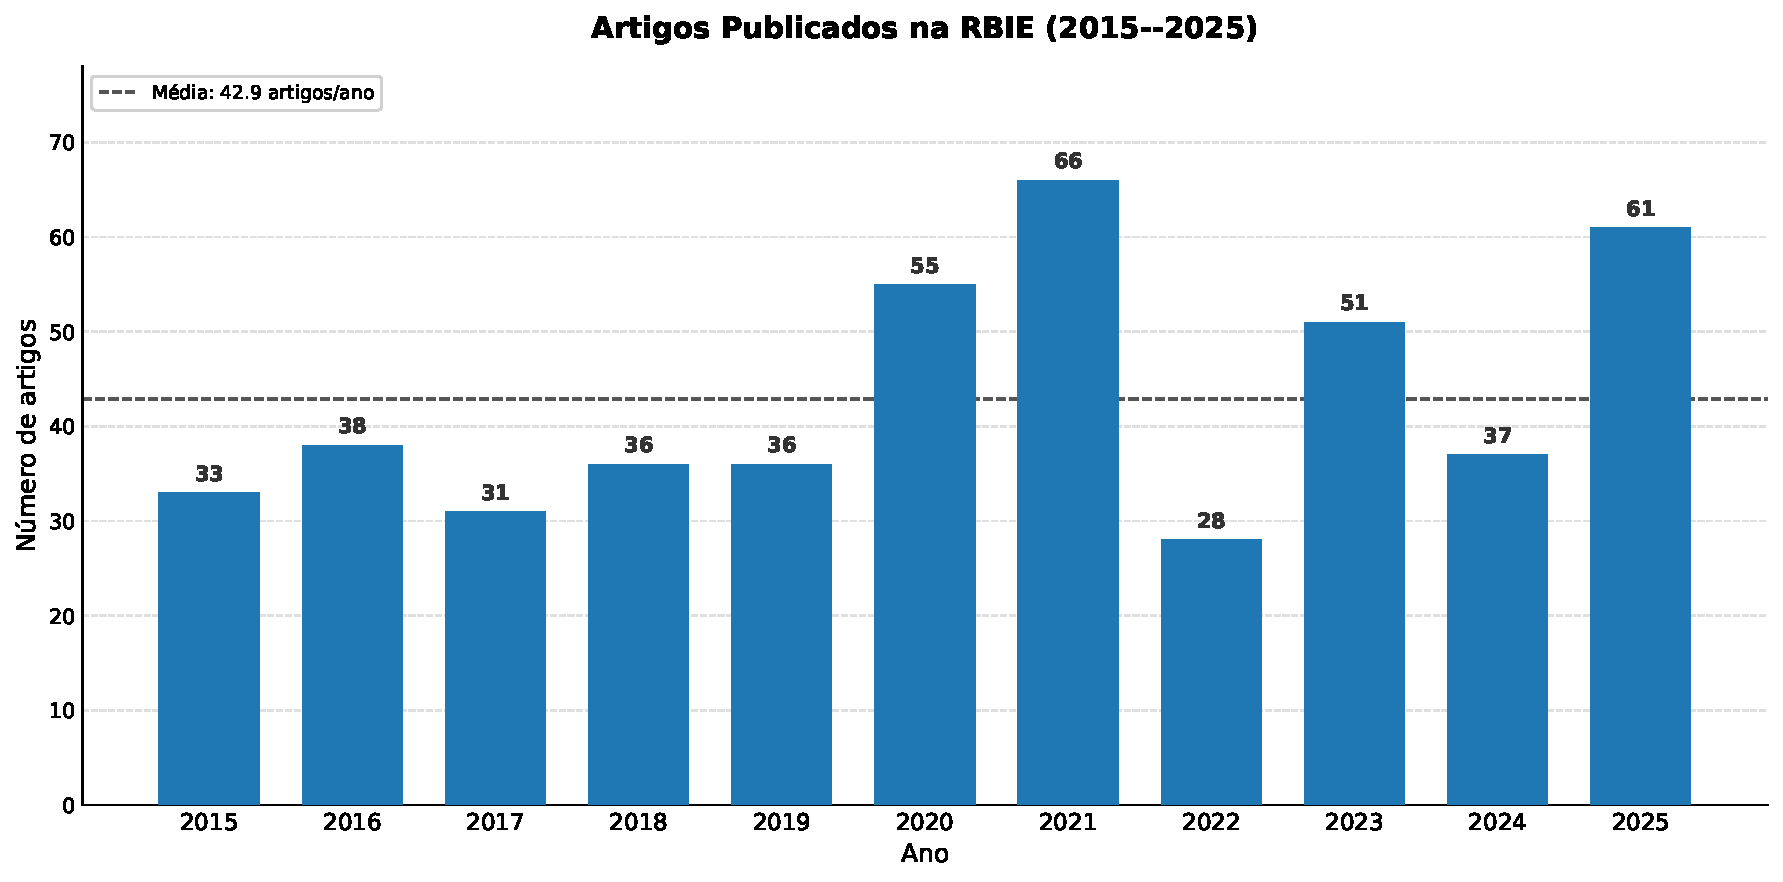
\includegraphics[width=\columnwidth,
      alt={Gráfico de líneas del número de artículos publicados en la RBIE por año. El eje horizontal indica los años y el eje vertical, la cantidad de artículos. La serie muestra una tendencia general de crecimiento a lo largo del período. Sustituya esta descripción por la de su figura.}]{img/rbie_artigos_por_ano.pdf}

    % Leyenda de la figura, mostrada en el PDF impreso:
    \caption{Ejemplo de leyenda de figura. Las leyendas de las figuras deben posicionarse abajo. Gráfico generado con la biblioteca Matplotlib en Python. Fuente de los datos: RBIE.}
    \label{fig:figura1coluna}
\end{figure}


\begin{figure*}
    \centering
    % ACCESIBILIDAD: vea la nota sobre la clave 'alt' en la figura de una columna arriba.
    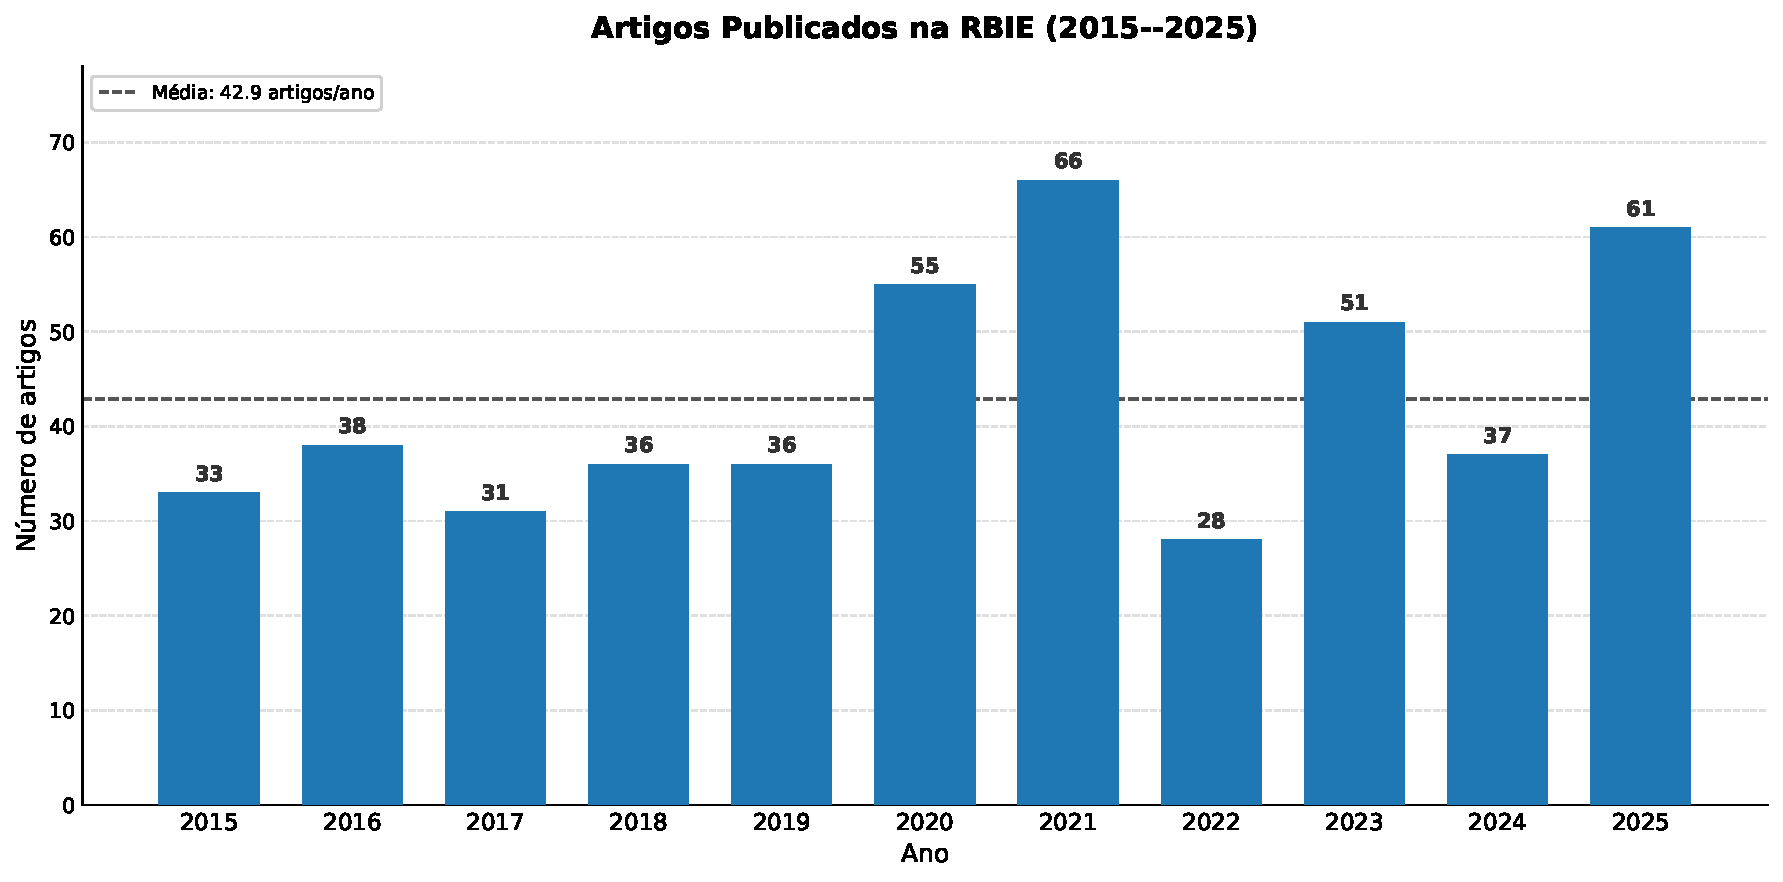
\includegraphics[width=.9\linewidth,
      alt={Gráfico de líneas del número de artículos publicados en la RBIE por año. El eje horizontal indica los años y el eje vertical, la cantidad de artículos. La serie muestra una tendencia general de crecimiento a lo largo del período. Sustituya esta descripción por la de su figura.}]{img/rbie_artigos_por_ano.pdf}
    \caption{Ejemplo de leyenda de figura. Las leyendas de las figuras deben posicionarse abajo. Gráfico generado con la biblioteca Matplotlib en Python. Fuente de los datos: RBIE.}
    \label{fig:figura2colunas}
\end{figure*}


\subsubsection{Recomendaciones Metodológicas}

\begin{enumerate}
  \item \textbf{Adecuación del tipo de figura a los datos.} El tipo de visualización debe ser coherente con la naturaleza de los datos; de lo contrario, distorsionará su interpretación. Por ejemplo, los gráficos de barras son adecuados para comparar categorías discretas; los gráficos de líneas, para mostrar tendencias a lo largo de una variable continua o temporal; los gráficos de dispersión, para relacionar dos variables cuantitativas.

  \item \textbf{Autonomía informativa.} La leyenda posicionada debajo de la figura debe ser suficiente para que se comprenda de forma independiente del texto. Los ejes, las series, los símbolos y los colores utilizados deben identificarse en la propia figura o en la leyenda.

  \item \textbf{Integridad de la representación visual.} La escala de los ejes debe comenzar en cero cuando se trate de cantidades absolutas, salvo que exista una justificación explícita. Las escalas truncadas o no lineales sin una advertencia explícita distorsionan la percepción de las diferencias entre los valores y constituyen un error metodológico.

  \item \textbf{Identificación de la fuente para datos secundarios.} Las figuras basadas en datos de otras fuentes deben indicar la referencia explícitamente en la leyenda. Las figuras reproducidas o adaptadas de otros trabajos deben indicar la fuente y, cuando corresponda, el permiso de uso.

  \item \textbf{Diagramas de proceso y de flujo.} Los diagramas de flujo, los diagramas de secuencia y los mapas conceptuales deben tener una notación coherente a lo largo del artículo.

   \item \textbf{Origen de los datos y herramienta de generación.} La leyenda o el texto del manuscrito debe identificar: (A) la fuente de la que se extrajeron los datos presentados en la figura; y (B) el software o la herramienta utilizada para generar la figura (por ejemplo, una biblioteca específica de R o Python). Cuando se utilice una herramienta de IA generativa para crear, modificar o mejorar la figura, esto debe declararse explícitamente en la ``Declaración sobre el uso de la inteligencia artificial (IA)'', ubicada al final del artículo, según lo exige el Código de Conducta para autores de la SBC \citeyearpar{SBC2024conduta_pt}. Las figuras generadas íntegramente por IA sin intervención metodológica de los autores (por ejemplo, diagramas o infografías producidos mediante un prompt) deben evitarse en artículos de investigación primaria, ya que no constituyen una representación verificable de datos empíricos. Cuando se utilicen con fines ilustrativos, deben identificarse como tales.

  \item \textbf{Figuras en revisiones sistemáticas.} En los artículos de revisión o mapeo sistemático, el diagrama de flujo de selección de estudios es un elemento obligatorio. Debe registrar el número de estudios en cada etapa del proceso de cribado, permitiendo que el lector verifique la transparencia del proceso de selección de estudios.
\end{enumerate}


\subsubsection{Errores que Evitar en las Figuras}

\begin{enumerate}
  \item \textbf{Figuras decorativas o redundantes.} Evite incluir figuras cuyo contenido ya esté plenamente cubierto por una tabla o por el texto. Cada figura debe añadir información o perspectiva que los demás elementos no ofrezcan.

  \item \textbf{Exceso de variables en una sola figura.} Las figuras con demasiadas series, colores o dimensiones simultáneas dificultan la extracción de conclusiones. Prefiera dividir las visualizaciones complejas en figuras más pequeñas y focalizadas.

  \item \textbf{Gráficos de sectores para cuatro o más categorías.} Los gráficos de sectores dificultan la comparación precisa entre porciones de tamaño y color similares. Para cuatro o más categorías, los gráficos de barras ofrecen mayor precisión perceptiva y deben preferirse.

  \item \textbf{Ausencia de barras de error en datos experimentales.} Los gráficos que presentan medias de datos experimentales sin indicar medidas de dispersión (desviación estándar, error estándar o intervalo de confianza) ocultan la variabilidad de los resultados.

  \item \textbf{Leyendas vagas.} Leyendas como ``Resultados del experimento'' no identifican el contenido de la figura. La leyenda debe describir, de forma autocontenida, lo que se muestra, sin que el lector tenga que recurrir directamente al texto para extraer el contexto.

  \item \textbf{Capturas de pantalla como sustituto de los datos.} Las capturas de pantalla de herramientas solo son aceptables cuando el objetivo es ilustrar la propia interfaz. Los datos numéricos extraídos de herramientas deben presentarse en tablas o gráficos construidos por los autores, no como imágenes de la salida del software.

  \item \textbf{Efectos tridimensionales en los gráficos.} No aplique efectos 3D (perspectiva, profundidad, sombra o extrusión) a los gráficos de barras, de sectores, de líneas o de dispersión. Distorsionan visualmente las proporciones entre los valores, dificultan la lectura de las magnitudes representadas y no aportan información al gráfico. La tridimensionalidad solo se justifica cuando los datos tienen efectivamente tres dimensiones analíticas que representar.
\end{enumerate}


\subsubsection{Recomendaciones sobre Fotografías de Personas}

La publicación de fotografías de participantes de investigación está regulada por las siguientes normas de protección y privacidad:

\begin{itemize}

  \item \textbf{En Brasil:}

  \begin{itemize}
    \item Ley General de Protección de Datos Personales (LGPD) \citep{LGPD2018};

    \item Estatuto del Niño y del Adolescente (ECA) \citep{ECA1990};

    \item Ley n.º 14.874/2024 \citep{brasil2024lei14874}, reglamentada por el Decreto n.º 12.651/2025 \citep{brasil2025decreto12651}, que regula la investigación con seres humanos e instituye el Sistema Nacional de Ética en Investigación con Seres Humanos, marco legal vigente desde 2024;

    \item Resoluciones CNS n.º 466/2012 \citep{cns2012resolucao466} y n.º 510/2016 \citep{cns2016resolucao510}, que permanecen válidas como referencia ética en la medida en que no entren en conflicto con el nuevo marco legal, durante el período de transición. La Resolución n.º 510/2016 trata específicamente de la investigación en Ciencias Humanas y Sociales, campo en el que se enmarca la mayoría de los estudios de Informática en la Educación; la Resolución n.º 466/2012 es el marco general y se aplica de forma subsidiaria.
  \end{itemize}

  \item \textbf{Internacionalmente:}

  \begin{itemize}
    \item Reglamento General de Protección de Datos de la Unión Europea (GDPR) \citep{GDPR2016};

    \item Directrices éticas de la \textit{American Psychological Association} (APA).
  \end{itemize}

\end{itemize}


Una fotografía de un participante de investigación no es un mero elemento decorativo del manuscrito. Es un dato personal sensible con implicaciones éticas, legales y humanas. Antes de incluir cualquier imagen que retrate a seres humanos, responda mentalmente a las siguientes preguntas:

\begin{enumerate}
  \item ¿Es esta imagen científicamente necesaria?

  \item ¿Tengo autorización documentada para publicarla?

  \item ¿La publicación preserva la dignidad de quienes aparecen en ella?
\end{enumerate}

Las recomendaciones siguientes orientan este proceso.

\begin{enumerate}
  \item \textbf{Necesidad científica de la imagen.} La inclusión de fotografías de personas debe justificarse por la contribución científica de la imagen al argumento del artículo. Ejemplo: las fotografías de participantes interactuando con herramientas o entornos de aprendizaje son pertinentes cuando el contexto espacial o conductual es relevante para el análisis. No deben incluirse fotografías de reuniones de equipo o meramente ilustrativas.

  \item \textbf{Consentimiento libre, informado y documentado.} La publicación de fotografías que permitan la identificación de adultos requiere un formulario de consentimiento informado (FCI) específico para el uso de imagen, distinto del FCI general de la investigación. El documento firmado debe ser conservado por los investigadores y estar disponible para su verificación por el equipo editorial de la RBIE.

  \item \textbf{Autorización de los tutores legales para fotografías de niños.} Para las imágenes de menores de 18 años, el consentimiento debe obtenerse de los padres o tutores legales, de acuerdo con el ECA (artículo 17). Se recomienda además obtener el asentimiento del niño, cuando su madurez lo permita, de acuerdo con la Resolución CNS n.º 466/2012 \citep{cns2012resolucao466}.

  \item \textbf{Anonimización cuando no se obtiene el consentimiento.} Cuando no sea posible obtener el consentimiento, o cuando exponer la identidad no sea necesario para el argumento científico, la fotografía debe anonimizarse antes del envío. Las técnicas aceptables incluyen difuminar u ocultar la región del rostro y otros elementos identificadores (tatuajes, uniformes con nombres, credenciales). La anonimización debe aplicarse a todas las personas identificables de la imagen, no solo al participante focal.

  \item \textbf{Declaración en el artículo.} Los autores deben declarar, en la sección de ``Declaraciones complementarias'' o en la sección de ``Metodología'', que se obtuvieron los consentimientos para el uso de imagen y que el estudio fue sometido y aprobado por el Comité de Ética en Investigación (CEP) competente. \textbf{Esta declaración es obligatoria para la publicación del estudio en la RBIE.} Como el sistema nacional de ética en investigación se encuentra en reorganización, se recomienda seguir las orientaciones vigentes del CEP de la institución de los autores en cuanto al flujo de envío y a la instancia responsable.

  \item \textbf{Atención a los contextos de vulnerabilidad.} Las fotografías que retratan a participantes en situación de vulnerabilidad (estudiantes con dificultades de aprendizaje, poblaciones indígenas, niños en riesgo) requieren un cuidado redoblado. En estos casos, incluso con consentimiento, los autores deben evaluar si publicar la imagen preserva la dignidad de los participantes y no los expone a riesgos adicionales derivados de la circulación del artículo.
\end{enumerate}


%------------------------------------------
\subsection{Ecuaciones}

Para insertar ecuaciones en el texto, recomendamos que los autores observen las siguientes orientaciones:

\begin{enumerate}
  \item \textbf{Numeración.} Numere todas las ecuaciones que se referencian en el texto. Si en el texto se utiliza una sola ecuación, entonces la numeración puede omitirse. Utilice el entorno \texttt{equation} para controlar la numeración automáticamente:

\begin{equation}
  \label{eq:fmeasure}
  F_1 = 2 \cdot \frac{\text{Precisión} \times \text{Exhaustividad}}
                     {\text{Precisión} + \text{Exhaustividad}}
\end{equation}

  \item \textbf{Referencia en el texto.} Toda ecuación debe referenciarse en el texto antes de su presentación; de lo contrario, será un mero elemento decorativo y, por tanto, prescindible. Utilice el comando \fakeverb{\eqref{etiqueta}}, que producirá, por ejemplo: ``como en la Ecuación~\eqref{eq:fmeasure}''. Observe que este comando, a diferencia de \fakeverb{\ref}, produce automáticamente un par de paréntesis alrededor del número de la ecuación.

  \item \textbf{Definición de las variables.} Defina todas las variables y símbolos inmediatamente después de la ecuación. Por ejemplo: ``donde $F_1$ es la media armónica entre la precisión y la exhaustividad''. No suponga que el lector conoce la notación adoptada.

  \item \textbf{Ecuaciones en línea.} Para expresiones cortas integradas en el texto corrido, utilice el modo matemático en línea (\fakeverb{$...$}). Por ejemplo: la precisión fue $\hat{y} = 0{,}87$. Reserve los entornos \texttt{equation} y \texttt{align} para expresiones que merezcan su propio énfasis.

  \item \textbf{Alineación de varias ecuaciones.} Al presentar un sistema de ecuaciones o una derivación paso a paso, utilice el entorno \texttt{align} para alinear los signos de igualdad:

\begin{align}
  \text{Precisión} &= \frac{VP}{VP + FP} \\
  \text{Exhaustividad} &= \frac{VP}{VP + FN}
\end{align}

  \item \textbf{Puntuación.} Las ecuaciones forman parte de la estructura sintáctica del texto y deben recibir la puntuación adecuada. Si la ecuación termina una frase, ciérrela con un punto. Si la frase continúa después de la ecuación, utilice una coma.

  \item \textbf{Notación coherente.} Mantenga la misma notación para la misma variable a lo largo de todo el artículo. Por ejemplo, las variables escalares deben escribirse en cursiva ($x$), los vectores en negrita ($\mathbf{v}$) y las matrices en negrita mayúscula ($\mathbf{A}$), según la convención matemática estándar \citep{AMS2021handbook, Higham2020handbook, Knuth1989mathematical}.
\end{enumerate}


\subsection{Código de Programación}

Recomendamos las siguientes orientaciones para presentar listados de código o pseudocódigo:

\begin{enumerate}

  \item \textbf{Entorno recomendado.} Recomendamos el paquete \texttt{minted}\footnote{\url{https://ctan.org/pkg/minted}} para mostrar fragmentos de código con resaltado de sintaxis. El paquete ya está cargado por la clase \texttt{rbie2026} y no necesita declararse en el preámbulo. El Listado~\ref{lst:exemplominted} ilustra una función en Python.


\begin{listing}[H]
    \caption{Ejemplo de código formateado con el paquete \texttt{minted}.}
    \label{lst:exemplominted}
    \begin{minted}{python}
def soma(a, b):
    return a + b
    \end{minted}
    \vspace{-12pt} % elimina el espacio innecesario entre el listado y su leyenda debajo
\end{listing}

  \item \textbf{Fragmentos cortos en línea.} Para insertar identificadores, palabras reservadas o expresiones cortas en medio del texto, elija el comando según el contenido:

  \begin{itemize}
    \item Para nombres simples, sin caracteres especiales de \LaTeX, use \fakeverb{\texttt{...}}. Ejemplo: ``la función \texttt{calcular\_media()} devuelve un valor de tipo \texttt{float}''.

    \item Para mostrar fragmentos que contengan caracteres especiales (barra invertida, llaves, guion bajo, almohadilla), use \fakeverb{\fakeverb{...}}, que evita escapar manualmente esos caracteres. A diferencia de \fakeverb{\verb||}, también funciona dentro de leyendas, notas al pie y celdas de tabla. Ejemplo: \fakeverb{\fakeverb{\citep[p.~15]{clave}}} produce \fakeverb{\citep[p.~15]{clave}}. El comando lo proporciona el paquete \texttt{codehigh}, ya cargado en el preámbulo; el único requisito es que las llaves internas al argumento estén balanceadas.
  \end{itemize}

  \item \textbf{Pseudocódigo.} Cuando el objetivo sea describir un algoritmo de forma independiente del lenguaje, prefiera el pseudocódigo a un fragmento de código real. En ese caso, adopte una notación coherente y declare las convenciones utilizadas en la leyenda o en el texto. El Algoritmo~\ref{alg:soma} ilustra un pseudocódigo.


\begin{algorithm}
    \caption{Algoritmo de suma}
    \label{alg:soma}
    \begin{algorithmic}[1]
        \State $s \gets a + b$
    \end{algorithmic}
\end{algorithm}


  \item \textbf{Leyenda y referencia.} La leyenda de los bloques de código debe posicionarse \textbf{abajo}, siguiendo la misma convención que las figuras.

  \item \textbf{Extensión del fragmento.} Incluya solo el fragmento de código estrictamente necesario para ilustrar el punto discutido en el texto. Evite reproducir archivos enteros o funciones extensas. En su lugar, ponga el código completo a disposición en un repositorio público, reportado en las ``Declaraciones complementarias'', en la sección de ``Disponibilidad de datos y materiales''.

  \item \textbf{Identificadores.} Adopte un estándar para los nombres de variables, funciones y comentarios a lo largo de todo el artículo. Para los artículos escritos en español, son preferibles los identificadores en español, salvo cuando el código reproduzca un artefacto real ya publicado en otro idioma.
\end{enumerate}


\subsection{Cajas de Texto Numeradas}

Las cajas de texto pueden ser útiles para controlar la numeración y la referencia de una secuencia de prompts, cadenas de búsqueda u otro artefacto en forma de texto corrido. La Caja~\ref{inputbox:prompt} muestra un ejemplo de cómo puede presentarse un prompt en un artículo de la RBIE.

Para insertar una caja en \LaTeX, utilice el entorno personalizado \texttt{inputbox}, construido sobre el paquete \texttt{tcolorbox}\footnote{\url{https://ctan.org/pkg/tcolorbox}}.

El texto de la caja debe escribirse en la fuente \textit{TeX Gyre Termes}, tamaño 9pt, alineación justificada, con interlineado sencillo, sin espaciado antes ni después del párrafo.


\begin{inputbox}{Ejemplo de leyenda de una caja de texto: prompt para la generación sintética de una actividad en un curso de programación. Fuente: elaboración propia. \label{inputbox:prompt}}
    Eres un docente que imparte un curso de \textbf{\textcolor{variablecolor}{\{ASIGNATURA\}}} y quieres construir una actividad práctica para tus estudiantes. Ten en cuenta que tus estudiantes no tienen necesariamente una base sólida en matemáticas ni en informática, por lo que el nivel de dificultad de la tarea debe ser \textbf{\textcolor{variablecolor}{\{INTERMEDIO\}}}. La actividad práctica debe estar compuesta por \textbf{\textcolor{variablecolor}{\{NUM\_TAREAS\}}} tareas. Formatea la salida en markdown.
     % \label{}
\end{inputbox}



%------------------------------------------
\section{Limitaciones de la Investigación}
\label{sec:limitations}

La declaración de las limitaciones de la investigación es un requisito de la integridad científica y debe presentarse de forma reflexiva, no defensiva. Para facilitar la comunicación, recomendamos adoptar la taxonomía de \cite{Wohlin2012}, ya que es ampliamente utilizada en la investigación empírica en Ingeniería de Software e Informática en la Educación. Comprende las siguientes dimensiones:

\begin{enumerate}
  \item \textbf{Validez interna.} Discuta los factores que puedan haber influido en los resultados de forma no controlada, como los efectos de maduración, el sesgo de selección de participantes, la contaminación entre grupos o la pérdida de muestra.

  \item \textbf{Validez externa.} Discuta los límites de generalización de los resultados, considerando el perfil de los participantes, la institución, el contexto cultural y el período en que se realizó el estudio. No reclame una generalización que los datos no sustenten.

  \item \textbf{Validez de constructo.} Discuta en qué medida los instrumentos utilizados miden realmente los constructos que pretenden medir. Para escalas adaptadas o traducidas, indique los procedimientos de validación adoptados.

  \item \textbf{Validez de conclusión.} Discuta aspectos relacionados con la potencia estadística del estudio, la fiabilidad de las medidas y la coherencia del proceso de análisis.
\end{enumerate}

Para las revisiones y mapeos sistemáticos, las limitaciones deben abordar además \citep{Kitchenham2023_SEGRESS_supp}: el posible sesgo de publicación, las limitaciones de las bases de datos consultadas, las restricciones de idioma aplicadas y la subjetividad inherente al proceso de extracción y síntesis de datos.



%------------------------------------------
\section{Ciencia Abierta, Reproducibilidad y Disponibilidad de Materiales}
\label{sec:openscience}

La RBIE fomenta la adopción de prácticas de ciencia abierta como una forma de aumentar la transparencia, la reproducibilidad y el impacto de la investigación publicada. Las orientaciones siguientes se aplican a las dos fases del proceso editorial.


\subsection{Fase de Envío}

A efectos de la revisión doblemente anonimizada, si su trabajo implica artefactos en repositorios, entonces adopte estas precauciones:

\begin{itemize}
    \item \textbf{Repositorios anonimizados.} Los materiales complementarios, los conjuntos de datos, el código fuente y los instrumentos de investigación deben ponerse a disposición a través de repositorios anonimizados, como \textit{Anonymous GitHub} (\url{https://anonymous.4open.science/}), para no comprometer el anonimato del envío.

    \item \textbf{Preregistros.} Si el estudio se preregistró en plataformas como OSF (\url{https://osf.io/}) o AsPredicted (\url{https://aspredicted.org/}), el enlace debe anonimizarse u omitirse en la versión enviada, y restaurarse en la versión final.

    \item \textbf{Datos sensibles.} Los datos que involucren a participantes humanos no deben ponerse a disposición pública sin el debido tratamiento ético. Verifique que el protocolo de recolección cumpla con la Ley n.º 14.874/2024 \citep{brasil2024lei14874} y el Decreto n.º 12.651/2025 \citep{brasil2025decreto12651}, con las Resoluciones CNS n.º 466/2012 \citep{cns2012resolucao466} y n.º 510/2016 \citep{cns2016resolucao510}, que siguen válidas en la medida en que no entren en conflicto con el nuevo marco legal, y con la LGPD \citep{LGPD2018}.
\end{itemize}


\subsection{Fase de Entrega de la Versión Final}

Tras las rondas de revisión y la aceptación del artículo para su publicación en la RBIE, elimine la anonimización de la autoría en la versión final. Además, ponga a disposición todos los materiales y artefactos necesarios para la reproducibilidad de la investigación en las Declaraciones del artículo, en la sección de ``Disponibilidad de datos y materiales'', observando las siguientes precauciones:

\begin{itemize}
    \item \textbf{Datos de investigación.} Ponga a disposición los conjuntos de datos utilizados en los análisis en repositorios de acceso abierto con la asignación de un DOI permanente, como Zenodo (\url{https://zenodo.org/}), OSF (\url{https://osf.io/}), Dryad (\url{https://datadryad.org/}), Figshare (\url{https://figshare.com/}) o un repositorio institucional relevante. Indique en la versión final del manuscrito el repositorio, el DOI y demás información relevante.

    \item \textbf{Código fuente y scripts.} Comparta el código de análisis, los scripts de procesamiento y las implementaciones en repositorios públicos (por ejemplo, GitHub, GitLab), preferiblemente con una licencia abierta explícita, como MIT, Apache 2.0 o CC BY 4.0.

    \item \textbf{Instrumentos de investigación.} Ponga a disposición los cuestionarios, los guiones de entrevista, las rúbricas de evaluación y demás instrumentos utilizados en la recolección de datos como material complementario, ya sea en el repositorio en línea del artículo o como apéndice del manuscrito.

    \item \textbf{Materiales de intervención.} Comparta las actividades, los ejercicios, los problemas y demás materiales pedagógicos descritos en el estudio de forma que permita la replicación de la investigación por otros grupos.

    \item \textbf{Reproducibilidad computacional.} Cuando la investigación implique análisis computacionales, utilice entornos reproducibles, como contenedores Docker, entornos Conda o cuadernos Jupyter, acompañados de instrucciones claras de ejecución.

    \item \textbf{Licenciamiento.} Todos los materiales puestos a disposición deben tener una licencia de uso explícita. Para datos y documentos, se recomienda la licencia Creative Commons CC BY 4.0; para el software, una licencia de código abierto reconocida por la OSI (\url{https://opensource.org/}).

    \item \textbf{Declaración de disponibilidad.} Al final del manuscrito, incluya la sección titulada \textit{Disponibilidad de datos y materiales}, indicando dónde pueden accederse los recursos, o justificando, cuando corresponda, la imposibilidad de compartirlos.

    % \item \textbf{Preprints.} El envío de preprints a servidores como SocArXiv (\url{https://osf.io/preprints/socarxiv}) o EdArXiv (\url{https://osf.io/preprints/edarxiv}) está permitido, siempre que el preprint no identifique a los autores durante el período de revisión anónima.
\end{itemize}

La adopción de estas prácticas contribuye a la calidad científica de los trabajos publicados y está alineada con las directrices internacionales de ciencia abierta:

\begin{itemize}
    \item Recomendación de la UNESCO sobre la Ciencia Abierta \citep{UNESCO2022es}; y
    \item Principios FAIR (\textit{Findable, Accessible, Interoperable, Reusable}) de la gestión de datos \citep{FAIRprinciples2016}.
\end{itemize}



%------------------------------------------
\section{Conclusión y Trabajos Futuros}
\label{sec:conclusion}

La conclusión debe retomar el problema investigado, sintetizar los principales hallazgos en relación con las preguntas de investigación y presentar las implicaciones prácticas y teóricas del trabajo. Recomendamos la siguiente organización:

\begin{enumerate}
  \item \textbf{Retomar el problema y el objetivo.} En uno o dos párrafos iniciales, recapitule el problema que motivó el estudio y el objetivo propuesto. No reproduzca literalmente fragmentos de la introducción.

  \item \textbf{Síntesis de los resultados.} Presente los principales hallazgos de forma integrada, respondiendo directamente a las preguntas de investigación. La conclusión no es el lugar para introducir nuevos datos o análisis no discutidos previamente.

  \item \textbf{Implicaciones pedagógicas.} Discuta las implicaciones de los resultados para la práctica docente, para el diseño de herramientas o para la investigación en el campo. Destaque la aplicabilidad práctica, la transferibilidad y el impacto de los hallazgos en la educación. Distinga, cuando sea pertinente, las implicaciones para los investigadores, los docentes y otros profesionales de la educación.

  \item \textbf{Trabajos futuros.} Indique las direcciones de investigación que abre el presente trabajo. Los trabajos futuros deben derivarse de forma natural de las limitaciones identificadas y de los resultados obtenidos, sin constituir una lista de deseos desconectada del estudio.
\end{enumerate}

Por último, esperamos que la información contenida en esta plantilla de artículos ayude en la preparación de su manuscrito. Si encuentra alguna inconsistencia o necesita más información, póngase en contacto con el equipo editorial de la RBIE.



%------------------------------------------
% Declaraciones obligatorias y opcionales que complementan el texto
\begin{declarations}

\begin{acknowledgements}
ESTA DECLARACIÓN ES OPCIONAL. Los nombres que figuran como autores de esta plantilla son un homenaje póstumo a tres investigadores que dedicaron su trayectoria al desarrollo de la Informática en la Educación en Brasil. Alexandre Ibrahim Direne (1960--2017), José Armando Valente (1948--2025) y Liane Margarida Rockenbach Tarouco (1947--2025) no participaron en la elaboración de esta plantilla y no son responsables de ninguna parte de su contenido. Toda la responsabilidad por el material presentado aquí recae en los editores de la RBIE.
\end{acknowledgements}

\begin{funding}
ESTA DECLARACIÓN ES OPCIONAL. Esta investigación fue financiada por lorem ipsum dolor sit amet, consectetur adipiscing elit.
\end{funding}

\begin{contributions}
ESTA DECLARACIÓN ES OBLIGATORIA. Los autores deben describir su contribución utilizando la Taxonomía CRediT\footnote{\url{https://credit.niso.org/}}, como en este ejemplo: AID contribuyó a la concepción de este estudio. JAV y LMRT realizaron los experimentos. AID es el principal contribuyente y redactor de este manuscrito. Todos los autores leyeron y aprobaron el manuscrito final.
\end{contributions}

\begin{interests}
ESTA DECLARACIÓN ES OBLIGATORIA. Si no hay conflictos de intereses, los autores deben declarar: ``Los autores declaran que no tienen conflictos de intereses''. En caso contrario, la declaración debe ser: ``Los autores declaran que tienen los siguientes conflictos de intereses: lorem ipsum dolor sit amet, consectetur adipiscing elit.''
\end{interests}

\begin{materials}
ESTA DECLARACIÓN ES OBLIGATORIA.
  Si los autores ponen sus datos o su código a disposición de forma abierta, la declaración debe ser: ``Los conjuntos de datos (o el software) generados o analizados durante el presente estudio están disponibles en \ldots''. En caso contrario, la declaración debe ser: ``Los conjuntos de datos (o el software) generados o analizados durante el presente estudio se pondrán a disposición previa solicitud''.
\end{materials}

\begin{aiusagedeclaration}
ESTA DECLARACIÓN ES OBLIGATORIA. En cumplimiento del Código de Conducta para autores de la SBC \citeyearpar{SBC2024conduta_pt}, ``el uso de herramientas y tecnologías de IA generativa para generar contenido, en la redacción o la revisión del contenido de los artículos, debe declararse explícitamente en el trabajo''. Los autores deben enumerar las herramientas y describir dónde se utilizaron, por ejemplo: redacción inicial, revisión del texto, generación de ideas, análisis de datos, traducción, creación de figuras/tablas, generación de scripts u otras etapas. ``Estas herramientas no pueden figurar como autores del artículo. El uso de tales herramientas no exime a los autores de la responsabilidad por todo su contenido, incluso en caso de que se identifique plagio''. Si no se utilizó ninguna herramienta de IA generativa en ninguna etapa del desarrollo del trabajo, indíquelo explícitamente.
\end{aiusagedeclaration}


\begin{furtherinformation}
ESTA DECLARACIÓN ES DESEABLE. Incluya información adicional relevante, como, por ejemplo, la aprobación por un Comité de Ética en Investigación. Si no hay nada que añadir, esta declaración puede eliminarse.

Para los artículos premiados, adapte esta declaración de ejemplo: Esta publicación es una versión extendida del mejor artículo del $<$nombre del evento$>$ ($<$SIGLA DEL EVENTO$>$ 20XX), titulado \textit{``Título del artículo original''}. DOI: \url{https://doi.org/xxxxx.xxxx}.

\end{furtherinformation}
\end{declarations}


%%%% Estilo bibliográfico
\bibliographystyle{apalike-sol}

%%%% Base de datos de referencias bibliográficas
\bibliography{refs}


%%%% Apéndices
\section*{Apéndice A}

Los apéndices y anexos son materiales complementarios que amplían o apoyan el contenido del artículo sin interrumpir el flujo de lectura. La distinción entre ambos tipos depende de la autoría:

\begin{itemize}
  \item \textbf{Apéndice (caso más común):} material elaborado por los propios autores, como cuestionarios desarrollados para la investigación, guiones de entrevista, protocolos experimentales, rúbricas de evaluación o descripciones detalladas de implementaciones.

  \item \textbf{Anexo:} un documento externo incorporado al artículo por referencia, como resoluciones normativas, formularios institucionales estandarizados o instrumentos validados producidos por terceros.
\end{itemize}

Todo apéndice o anexo debe referenciarse en el cuerpo del texto. Los materiales que no se mencionen en el texto deben omitirse. Los apéndices y anexos deben aparecer después de las referencias bibliográficas, sin iniciar una nueva página, identificados por una letra mayúscula secuencial: Apéndice~A, Apéndice~B, Anexo~A, Anexo~B.

\end{document}
